\label{5_resultados}

\section{Parâmetros analisados}

Como um AG trabalha com tentativa-e-erro, não há uma geração exata para a qual pode ser prevista uma determinada solução (ou proximidade à solução). Para se analisar a evolução dos indivíduos ao longo das gerações, este trabalho focou em analisar os seguintes parâmetros:

\begin{itemize}
	\item Valor mínimo de fitness em um indivíduo;
	\item Valor máximo de fitness em um indivíduo;
	\item Valor médio de fitness entre todos os indivíduos;
	\item Desvio padrão dos valores de fitness.
\end{itemize}

O desvio padrão utilizado aqui foi o amostral, dado por:

\begin{equation}
	\sigma = \sqrt{\frac{1}{N-1} \sum_{i=1}^N (x_i - \overline{x})^2}
\end{equation}

Os gráficos criados tiveram como base uma única simulação do AG para o problema e parâmetros de entrada escolhidos. Não é possível ter expectativas de valores ou gerações, uma vez que o AG trabalha com tentativa-e-erro, então criá-las ou assumi-las seria difícil de quantizar.

Como já foi comentado antes, se não for mencionado o contrário (mesmo para o caso adaptativo), utilizou-se 0.9 para $p_c$ e 0.01 para $p_m$. Todas as execuções utilizaram 100 indivíduos, 200 gerações e elitismo do melhor indivíduo. Se um problema convergiu completamente para a melhor solução antes das 200 gerações completarem, os gráficos foram reduzidos para melhor visualização, uma vez que os pontos extras não trariam novas informações para nós.

As simulações feitas com uso do AGA foram utilizadas para comparação com a implementação estática do AG. Além disso, foi avaliado o comportamento adaptativo de $p_m$ ao longo das gerações.

\section{OneMax Booleano}

\subsection{Caso Estático}

Este problema foi considerado simples de ser resolvido por um AG, uma vez que poucas mutações em um gene já permitem que ele ficasse igual a 1. A figura \ref{fig:onemax_boolean} demonstra exatamente isso, com convergência completa dos indivíduos para a solução ótima após 93 gerações, sendo que a própria solução ótima foi encontrada com a melhor solução aparecendo após 78 gerações.

\begin{figure}[ht!]
    \centering 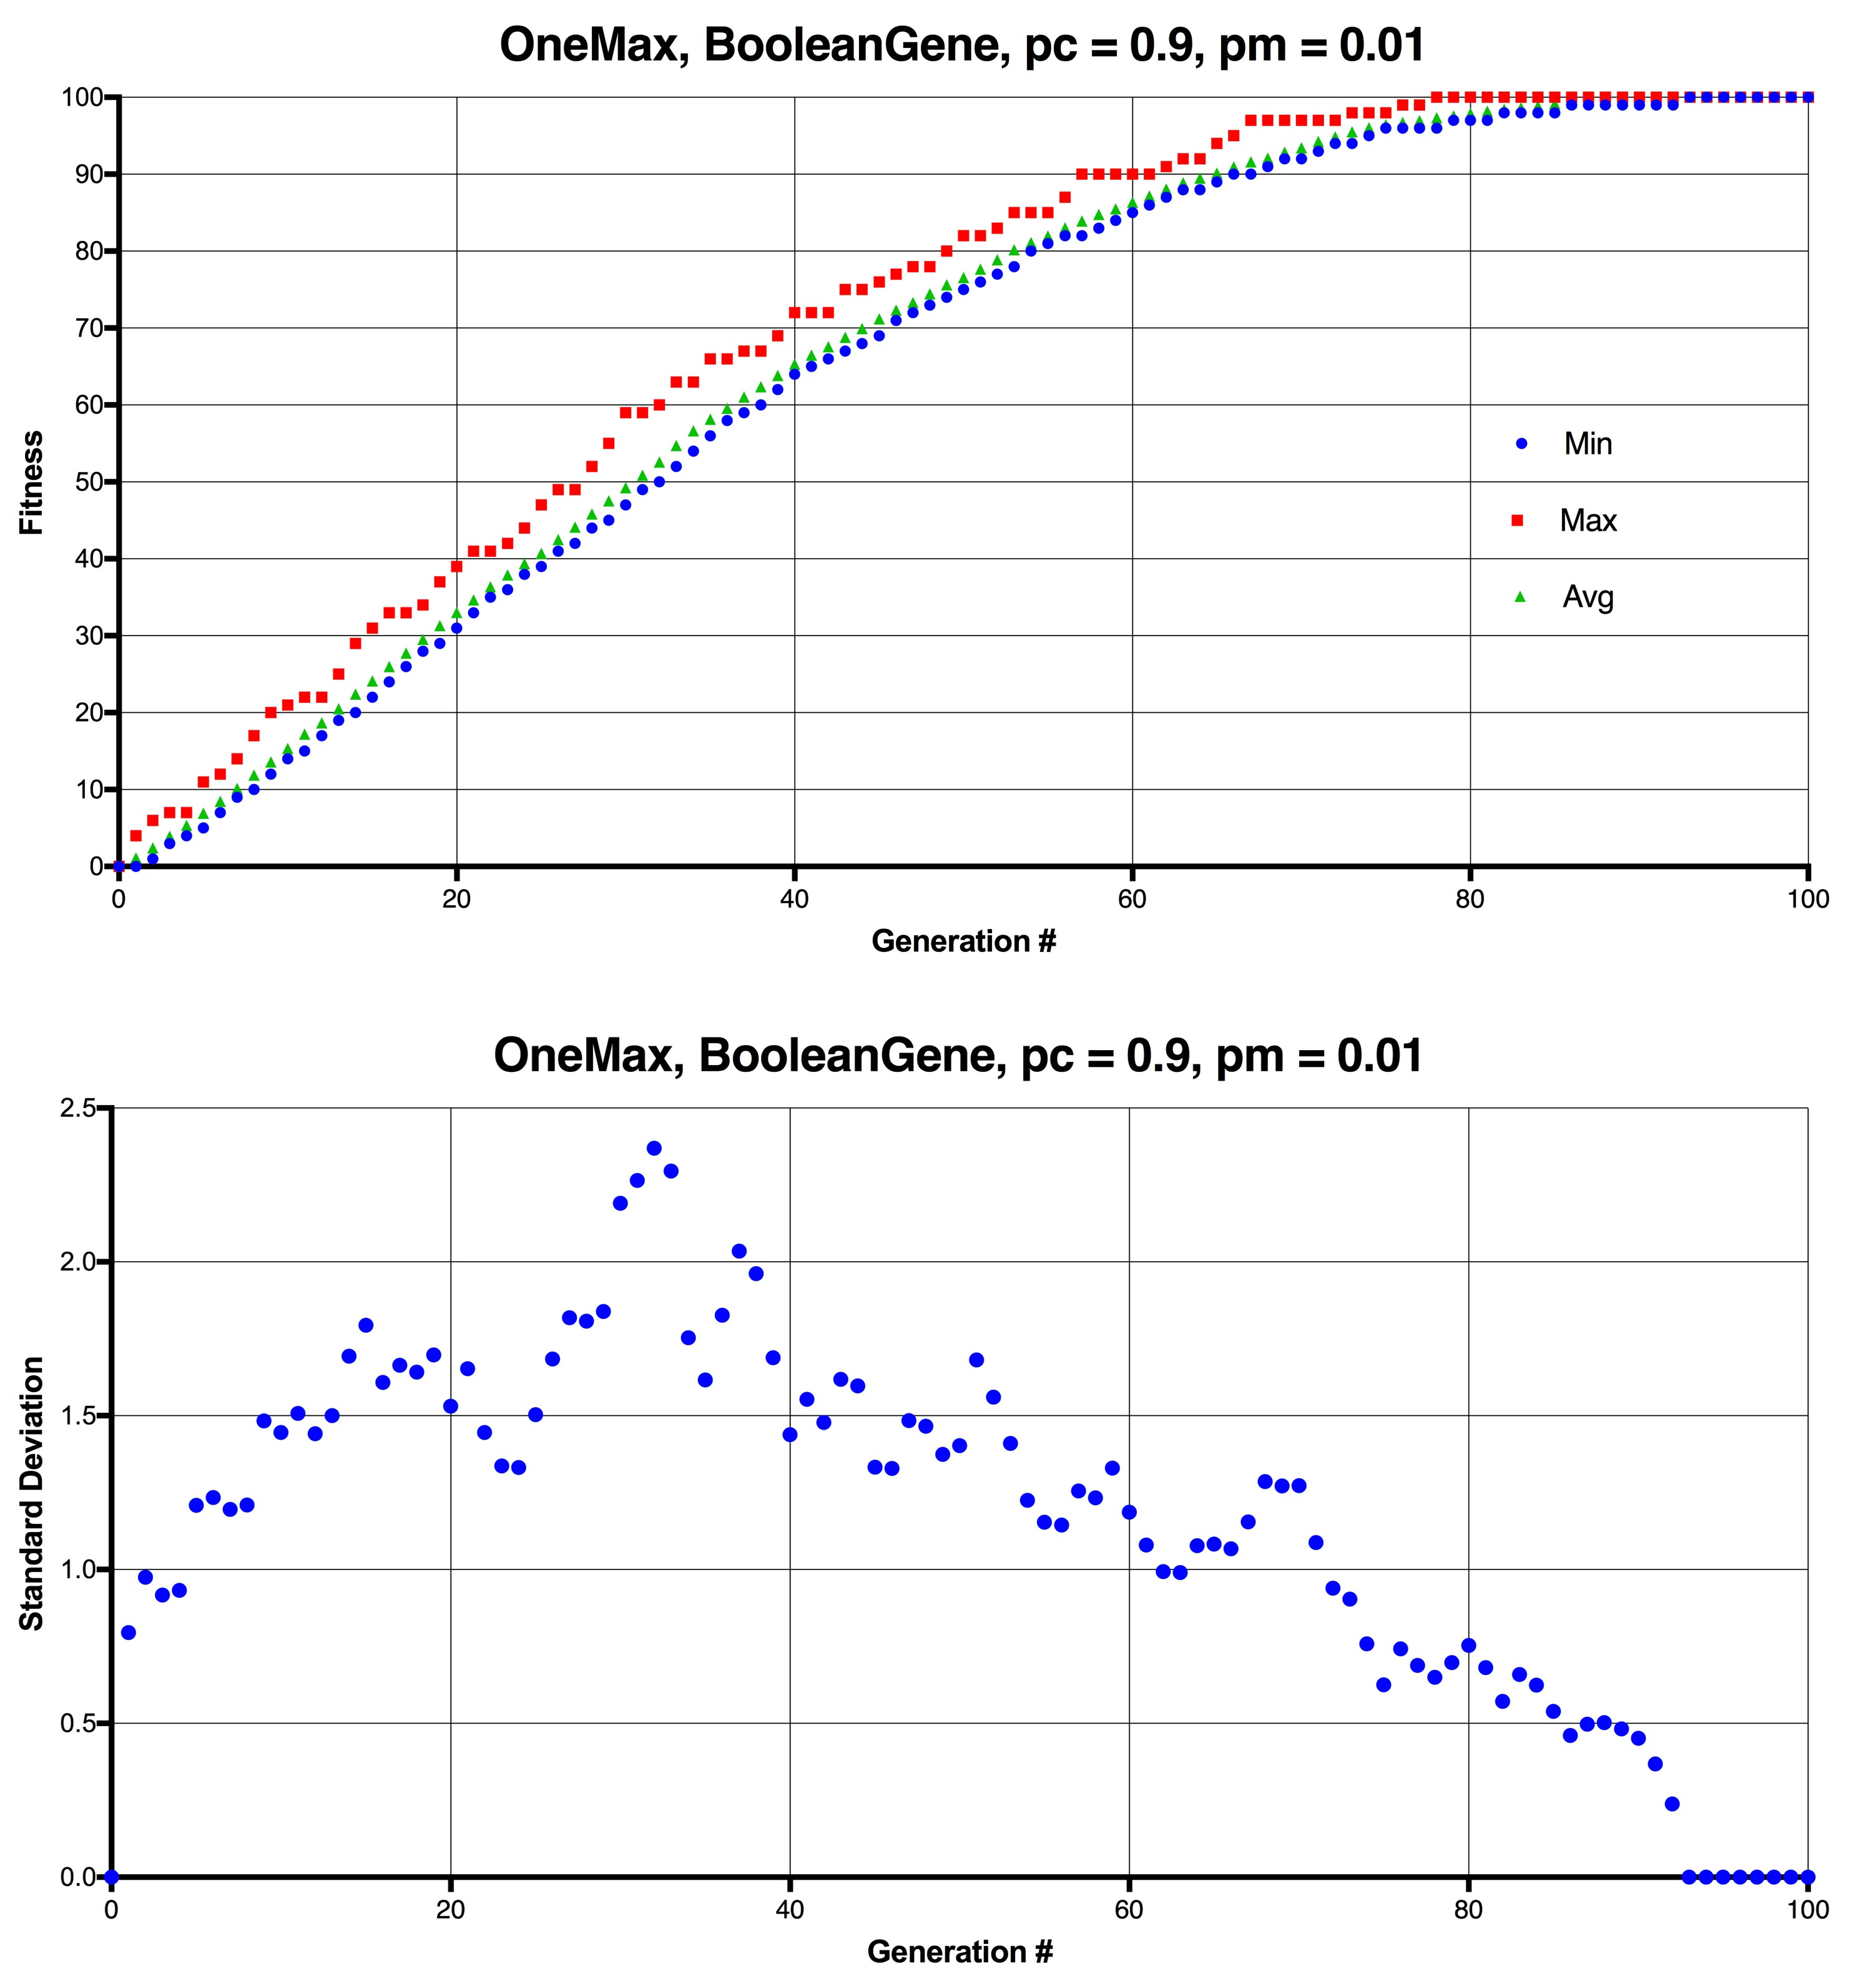
\includegraphics[width=1.0\textwidth]{onemax_boolean.jpg}
    \caption{Evolução do fitness para o problema do OneMax Booleano mostrando mínimo, máximo, valor médio e desvio padrão ($p_c=0.9$, $p_m=0.01$). Foram necessárias 78 gerações para que a solução ótima aparecesse, e 93 gerações para que a população inteira convergisse para ela.}
    \label{fig:onemax_boolean}
\end{figure}

O comportamento estático para os valores padronizados de $p_c$ e $p_m$ mostrou um crescimento aproximadamente linear dos valores de fitness, tanto para o pior quanto para o melhor indivíduo. Isso demonstra que tais valores demonstram um crescimento equilibrado da população, e a mutação existente é suficiente para evoluir os indivíduos.

\subsection{Caso Adaptativo}

Com o AGA ativado, ficou bem mais complicado para o OneMax atingir a solução ótima. Como mostrado na figura \ref{fig:onemax_boolean_adaptive}, foram necessárias 140 gerações para que o melhor indivíduo atingisse a solução ótima, e a média dos valores de fitness oscilou entre 98 e 99 para as últimas gerações. Em termos de desvio padrão, o valor nunca passou de 2.0 (de um máximo de 100), o que nos diz que a população não se dispersou completamente pelo efeito adaptativo.

\begin{figure}[ht!]
    \centering 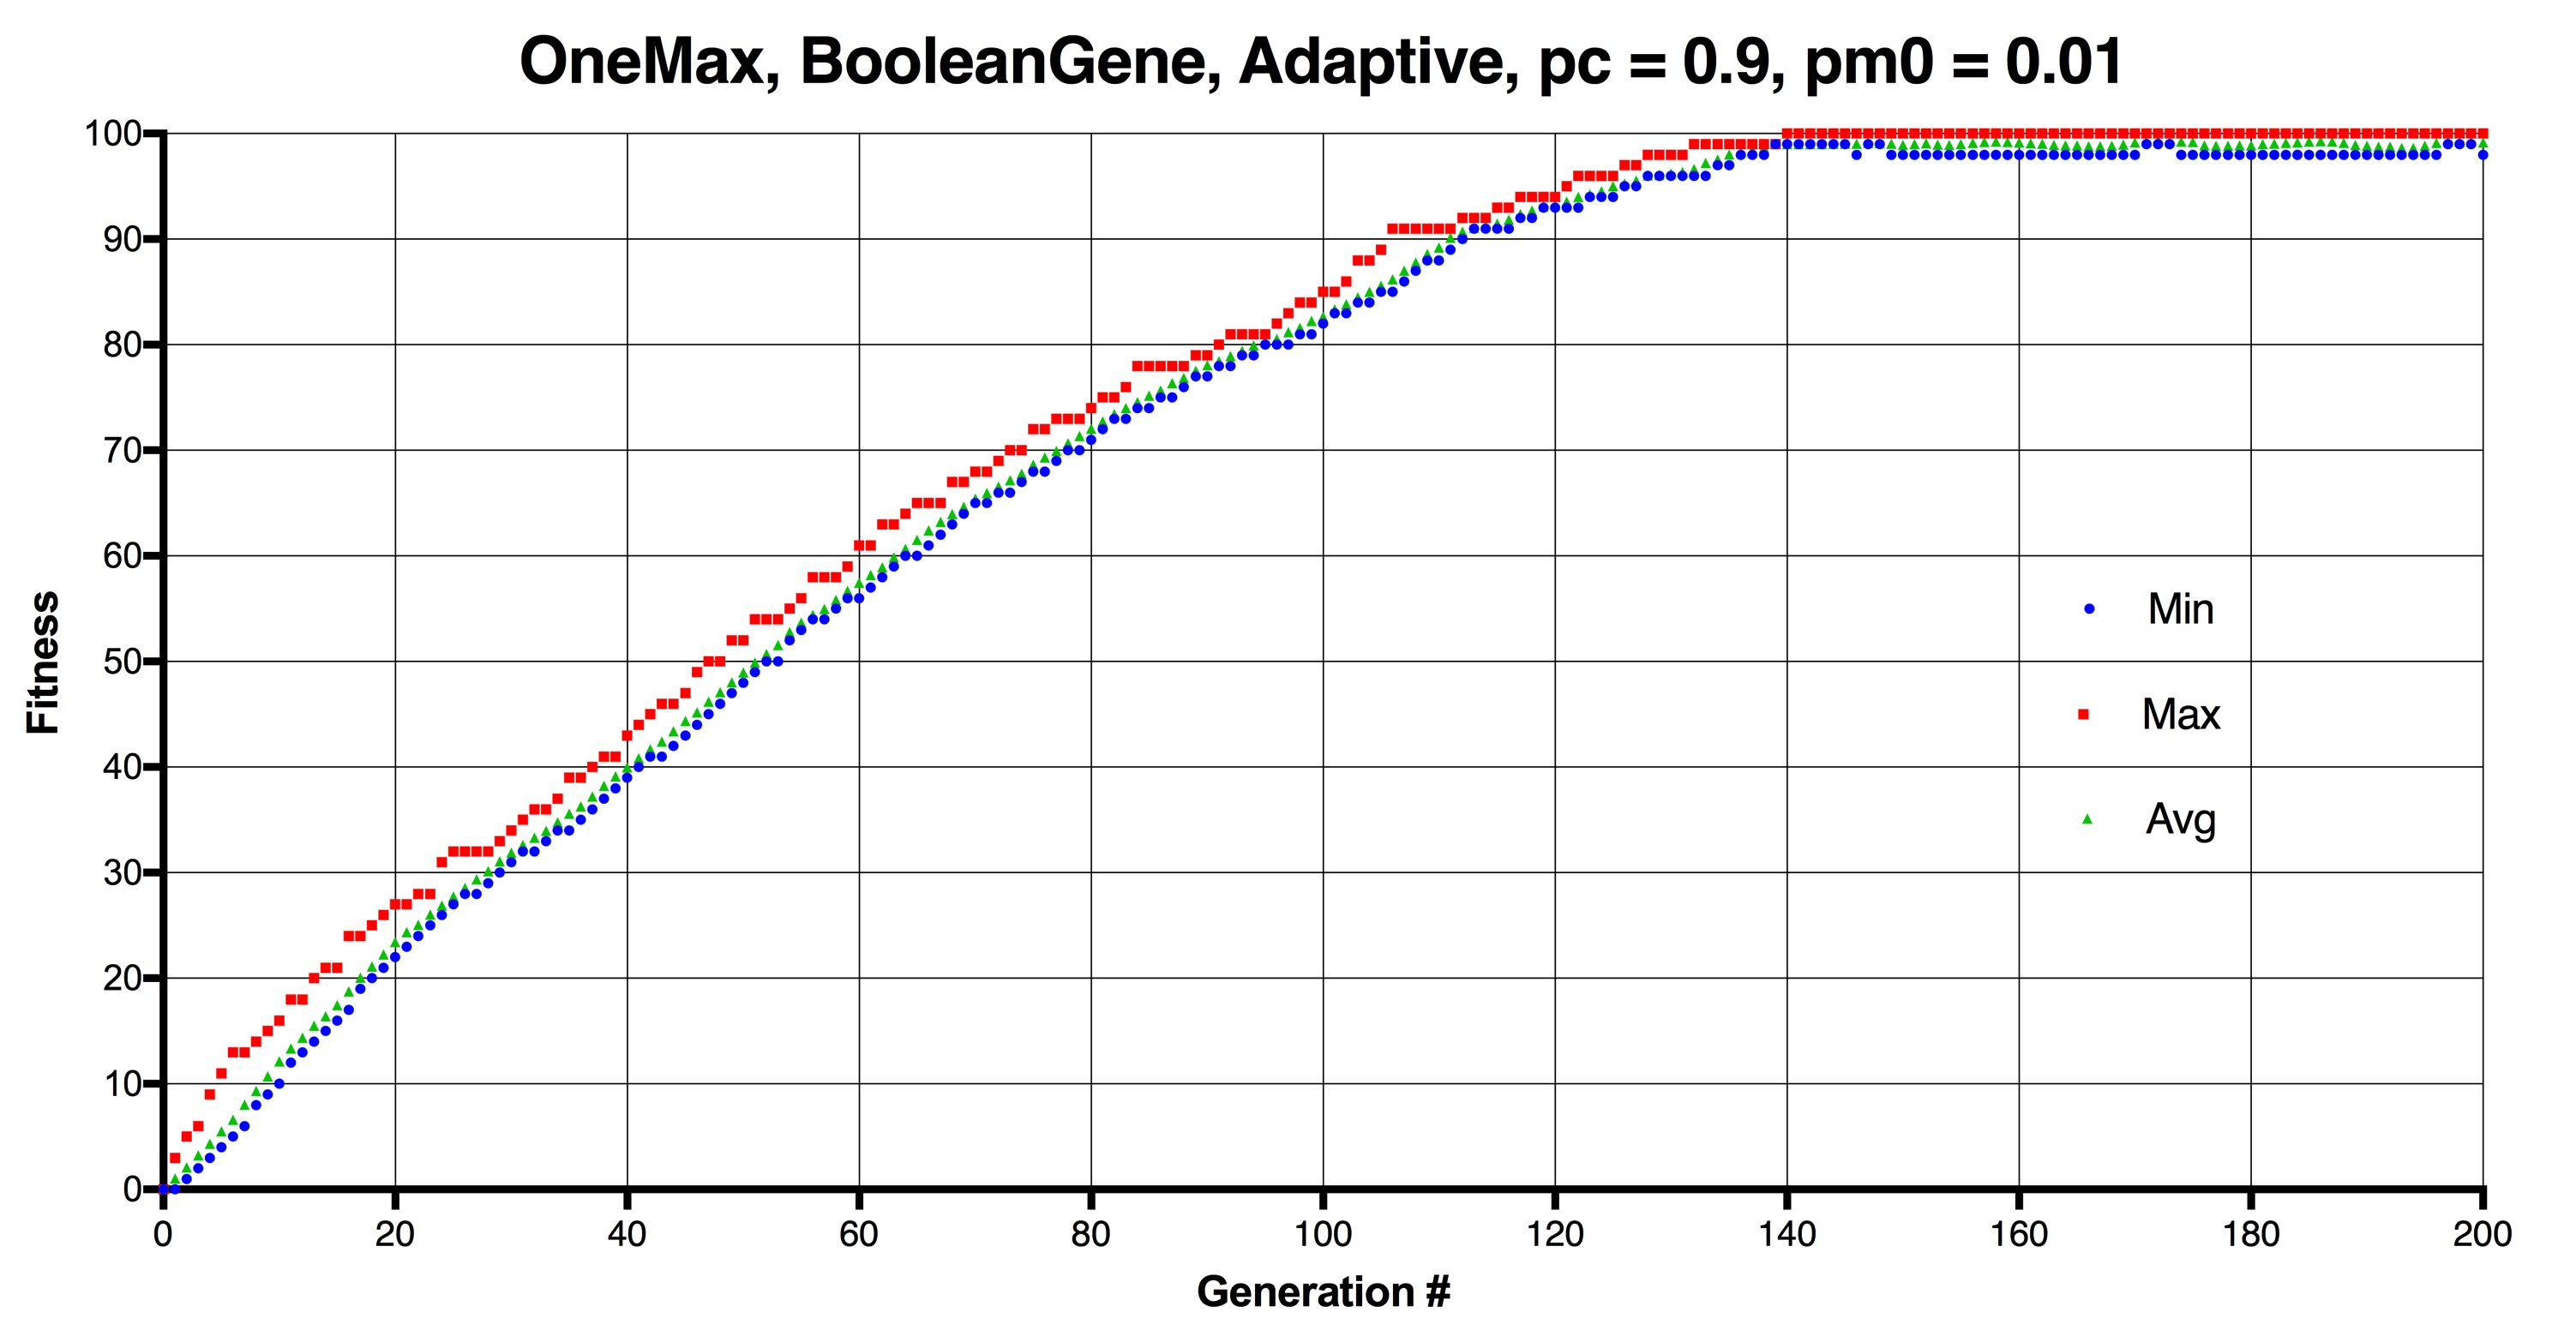
\includegraphics[width=1.0\textwidth]{onemax_boolean_adaptive.jpg}
    \caption{Evolução do fitness para o problema do OneMax Booleano Adaptativo mostrando mínimo, máximo, valor médio e desvio padrão ($p_c=0.9$, ${p_m}_0=0.01$). Foram necessárias 140 gerações para que um indivíduo encontrasse a solução ótima.}
    \label{fig:onemax_boolean_adaptive}
\end{figure}

Um efeito interessante pode ser visto na figura \ref{fig:onemax_boolean_adaptive_pm} com relação à evolução de $p_m$ e ${p_m}_0$. É possível ver que as primeiras gerações ainda eram muito dispersas, o que fez com que $p_m$ começasse a cair. No entanto, como mencionado antes, um valor baixo de $p_m$ se mostrou mais do que suficiente para que a população do caso estático fosse capaz de encontrar a solução ótima.

\begin{figure}[ht!]
    \centering 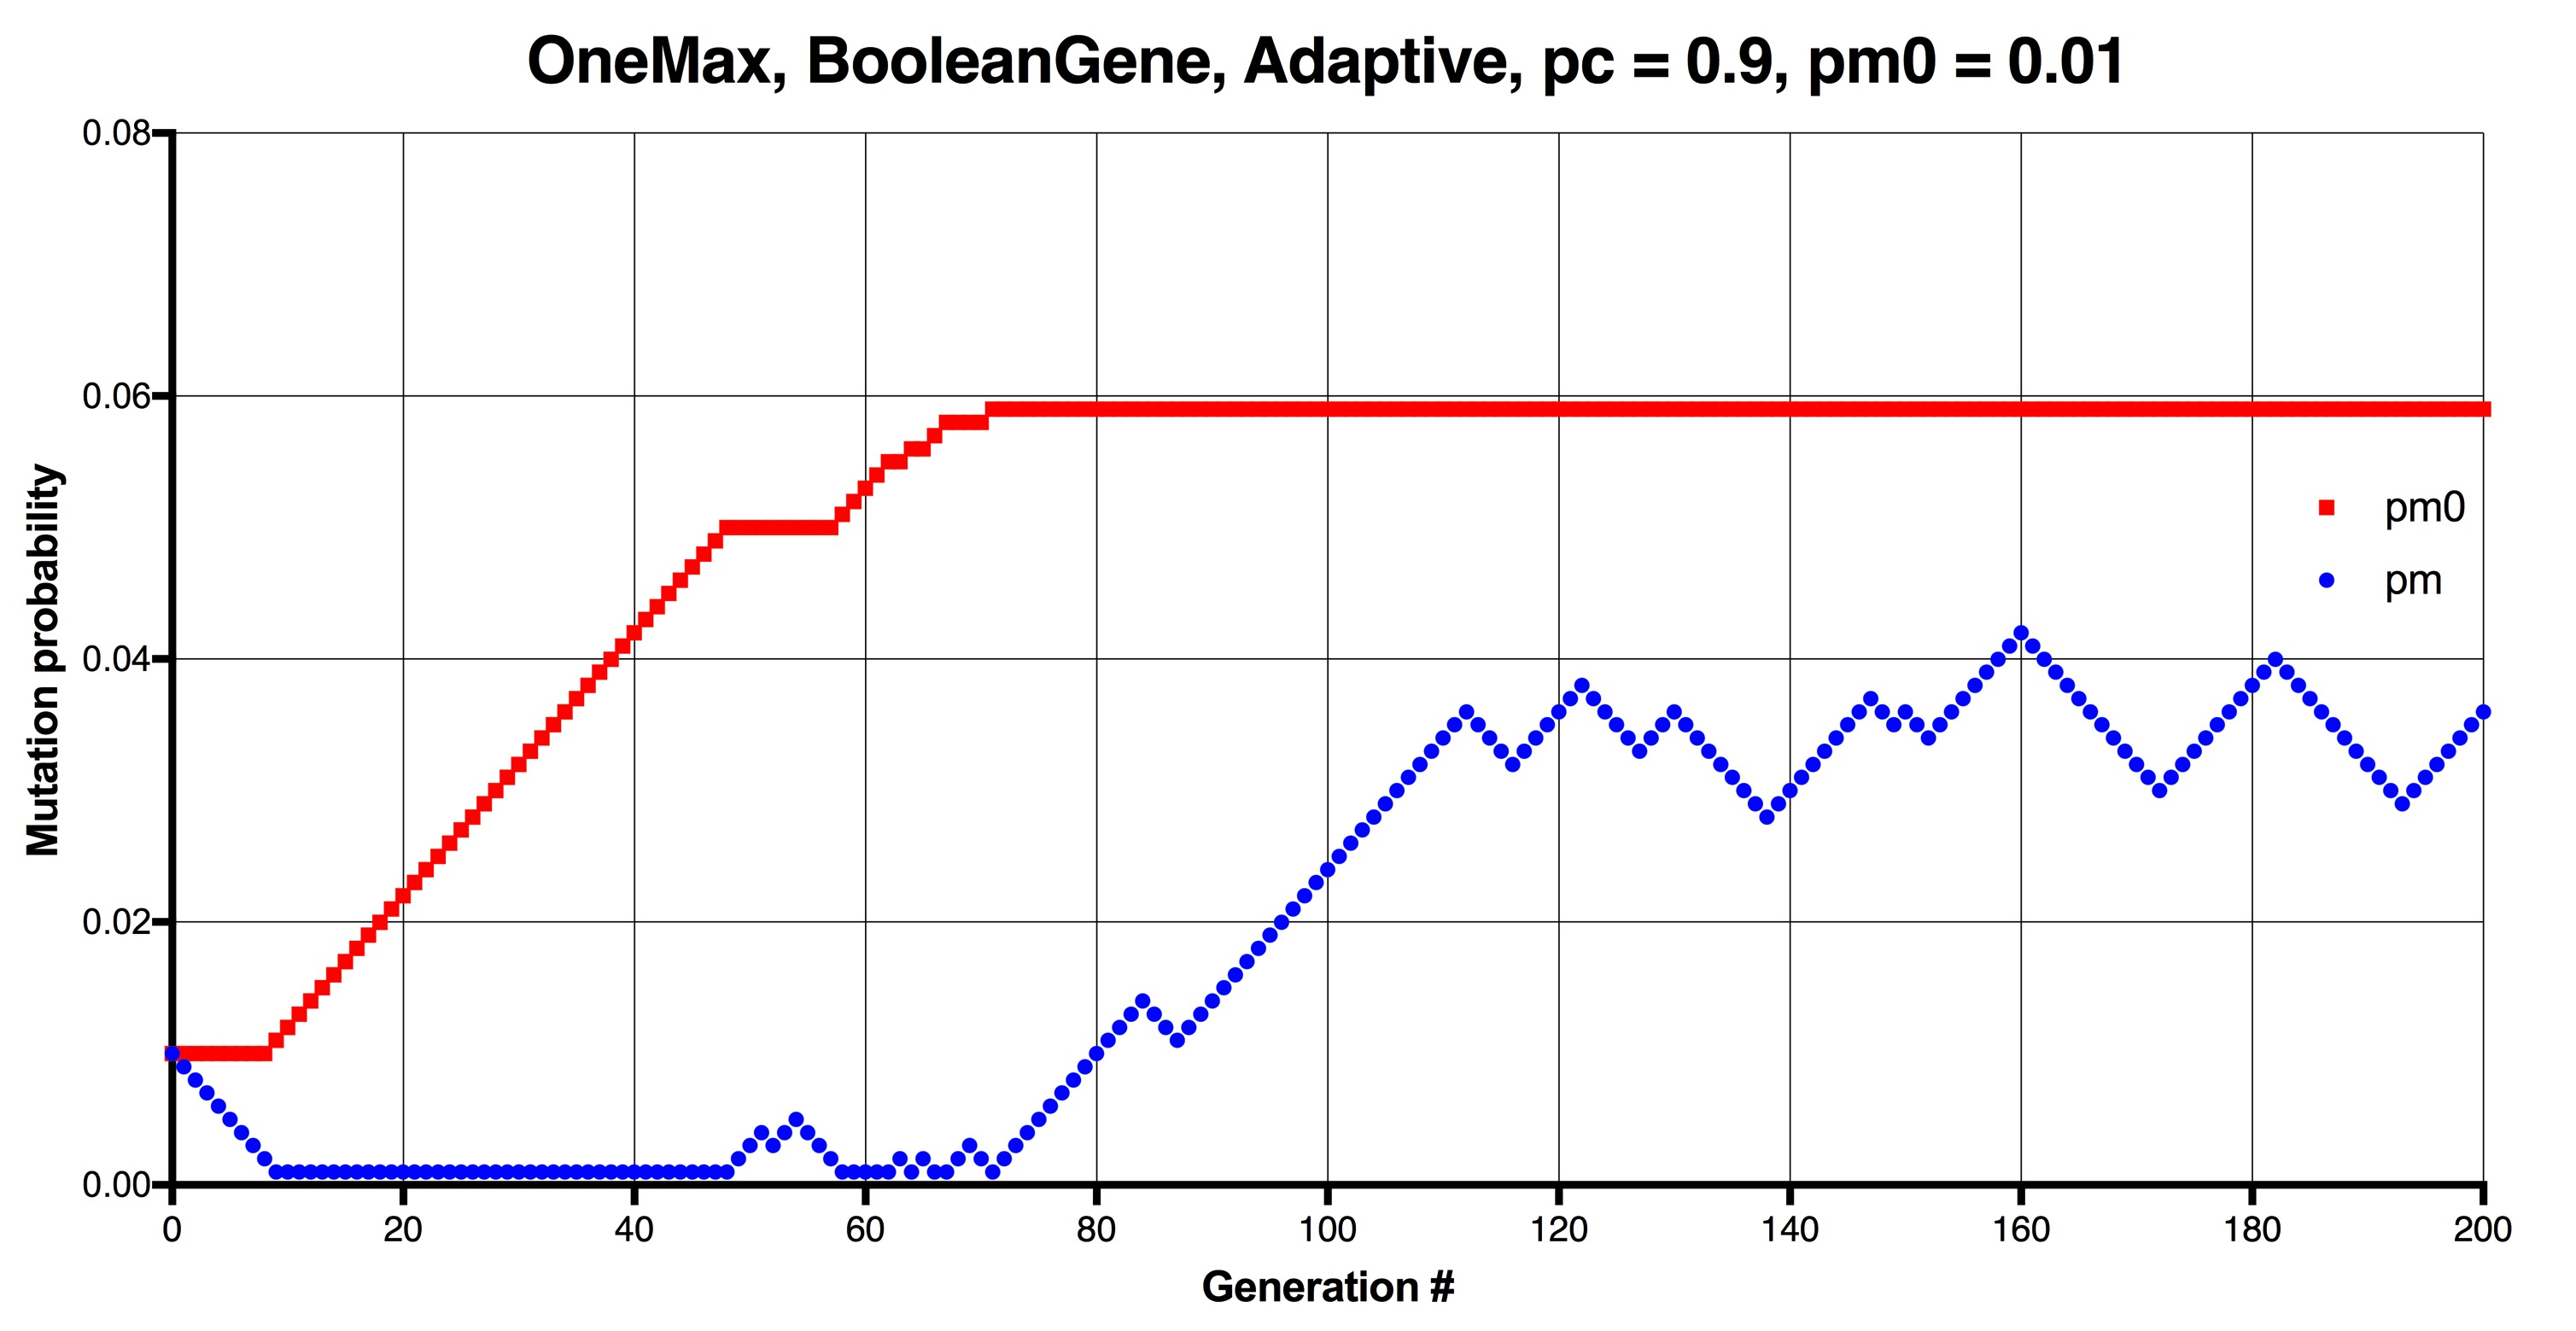
\includegraphics[width=1.0\textwidth]{onemax_boolean_adaptive_pm.jpg}
    \caption{Evolução da probabilidade de mutação $p_m$ ao longo das gerações, juntamente com o desvio do melhor valor de fitness com relação à média ($p_c=0.9$, ${p_m}_0=0.01$).}
    \label{fig:onemax_boolean_adaptive_pm}
\end{figure}

Por conta disso, ${p_m}_0$ começou a aumentar enquanto a população evoluía e ficava mais homogênea. O AGA, para uma população homogênea, interpreta isso como se a população tivesse travado em uma solução. Por conta disso, após cerca de 70 gerações, a homogeneização da população e o aumento de ${p_m}_0$ se encontraram, e $p_m$ começou a aumentar.

Quando $p_m$ parou de crescer (por volta de 110 gerações), ele estabilizou em torno de um valor mais alto que o inicial (por volta de 0.03). Tal aumento (tanto de $p_m$ quanto de ${p_m}_0$) se mostrou suficiente para que a população fosse incapaz de convergir conjuntamente para a solução ótima.

Foi possível tirar desta simulação que, mesmo que o intuito inicial deste AGA tivesse sido o de fugir de momentos em que o AG travasse em uma solução, ele veio com um custo, que foi o de evitar que a população fosse capaz de convergir conjuntamente para a solução ótima. Se o intuito de usar o AG for o de encontrar uma boa solução no final, esse custo é baixo.

Os dados de interesse vindos destas simulações podem ser encontrados na tabela \ref{tab:onemax_boolean}.

\begin{table}
\caption{Dados coletados do problema do OneMax Booleano ($p_m = 0.01$).}
\label{tab:onemax_boolean}

\center
\begin{tabular}{|c|cc|}
	\hline
	Algoritmo analisado (AG = caso estático)	& AG		& AGA		\\
	\hline
	Solução ótima encontrada?					& Sim		& Sim		\\
	Gerações p/solução ótima					& $78$		& $140$		\\
	Convergência da população (gerações)		& $93$		& $--$		\\
	Fitness médio após 100 gerações				& $100$		& $82.67$	\\
	Fitness médio após 200 gerações 			& $100$		& $99.17$	\\
	Valor final de $p_m$						& $0.01$ 	& $0.019$	\\
	Valor mínimo de $p_m$						& $0.01$	& $0.001$	\\
	Valor máximo de $p_m$						& $0.01$	& $0.021$	\\
	Valor médio de $p_m$						& $0.01$	& $0.00594$	\\
	Valor médio de $p_m$ (últimas 100 gerações)	& $0.01$	& $0.0105$	\\
	\hline
\end{tabular}
\end{table}

\section{OneMax Real}

Para o OneMax Real, é virtualmente impossível chegar ao valor máximo de fitness (100.0), uma vez que a mutação para um número aleatório trabalha no intervalo [0, 1). Por conta disso, as análises feitas aqui focaram no comportamento da curva e na diferença de comportamento frente aos resultados do OneMax Booleano.

\subsection{Caso Estático}

Para o OneMax Real, foi possível ver, na figura \ref{fig:onemax_real}, que a população, mesmo não sendo capaz de atingir o fitness máximo, conseguiu se homogeneizar e continuar crescendo ao longo das gerações, o que foi demonstrado também pela queda do desvio padrão.

\begin{figure}[ht!]
    \centering 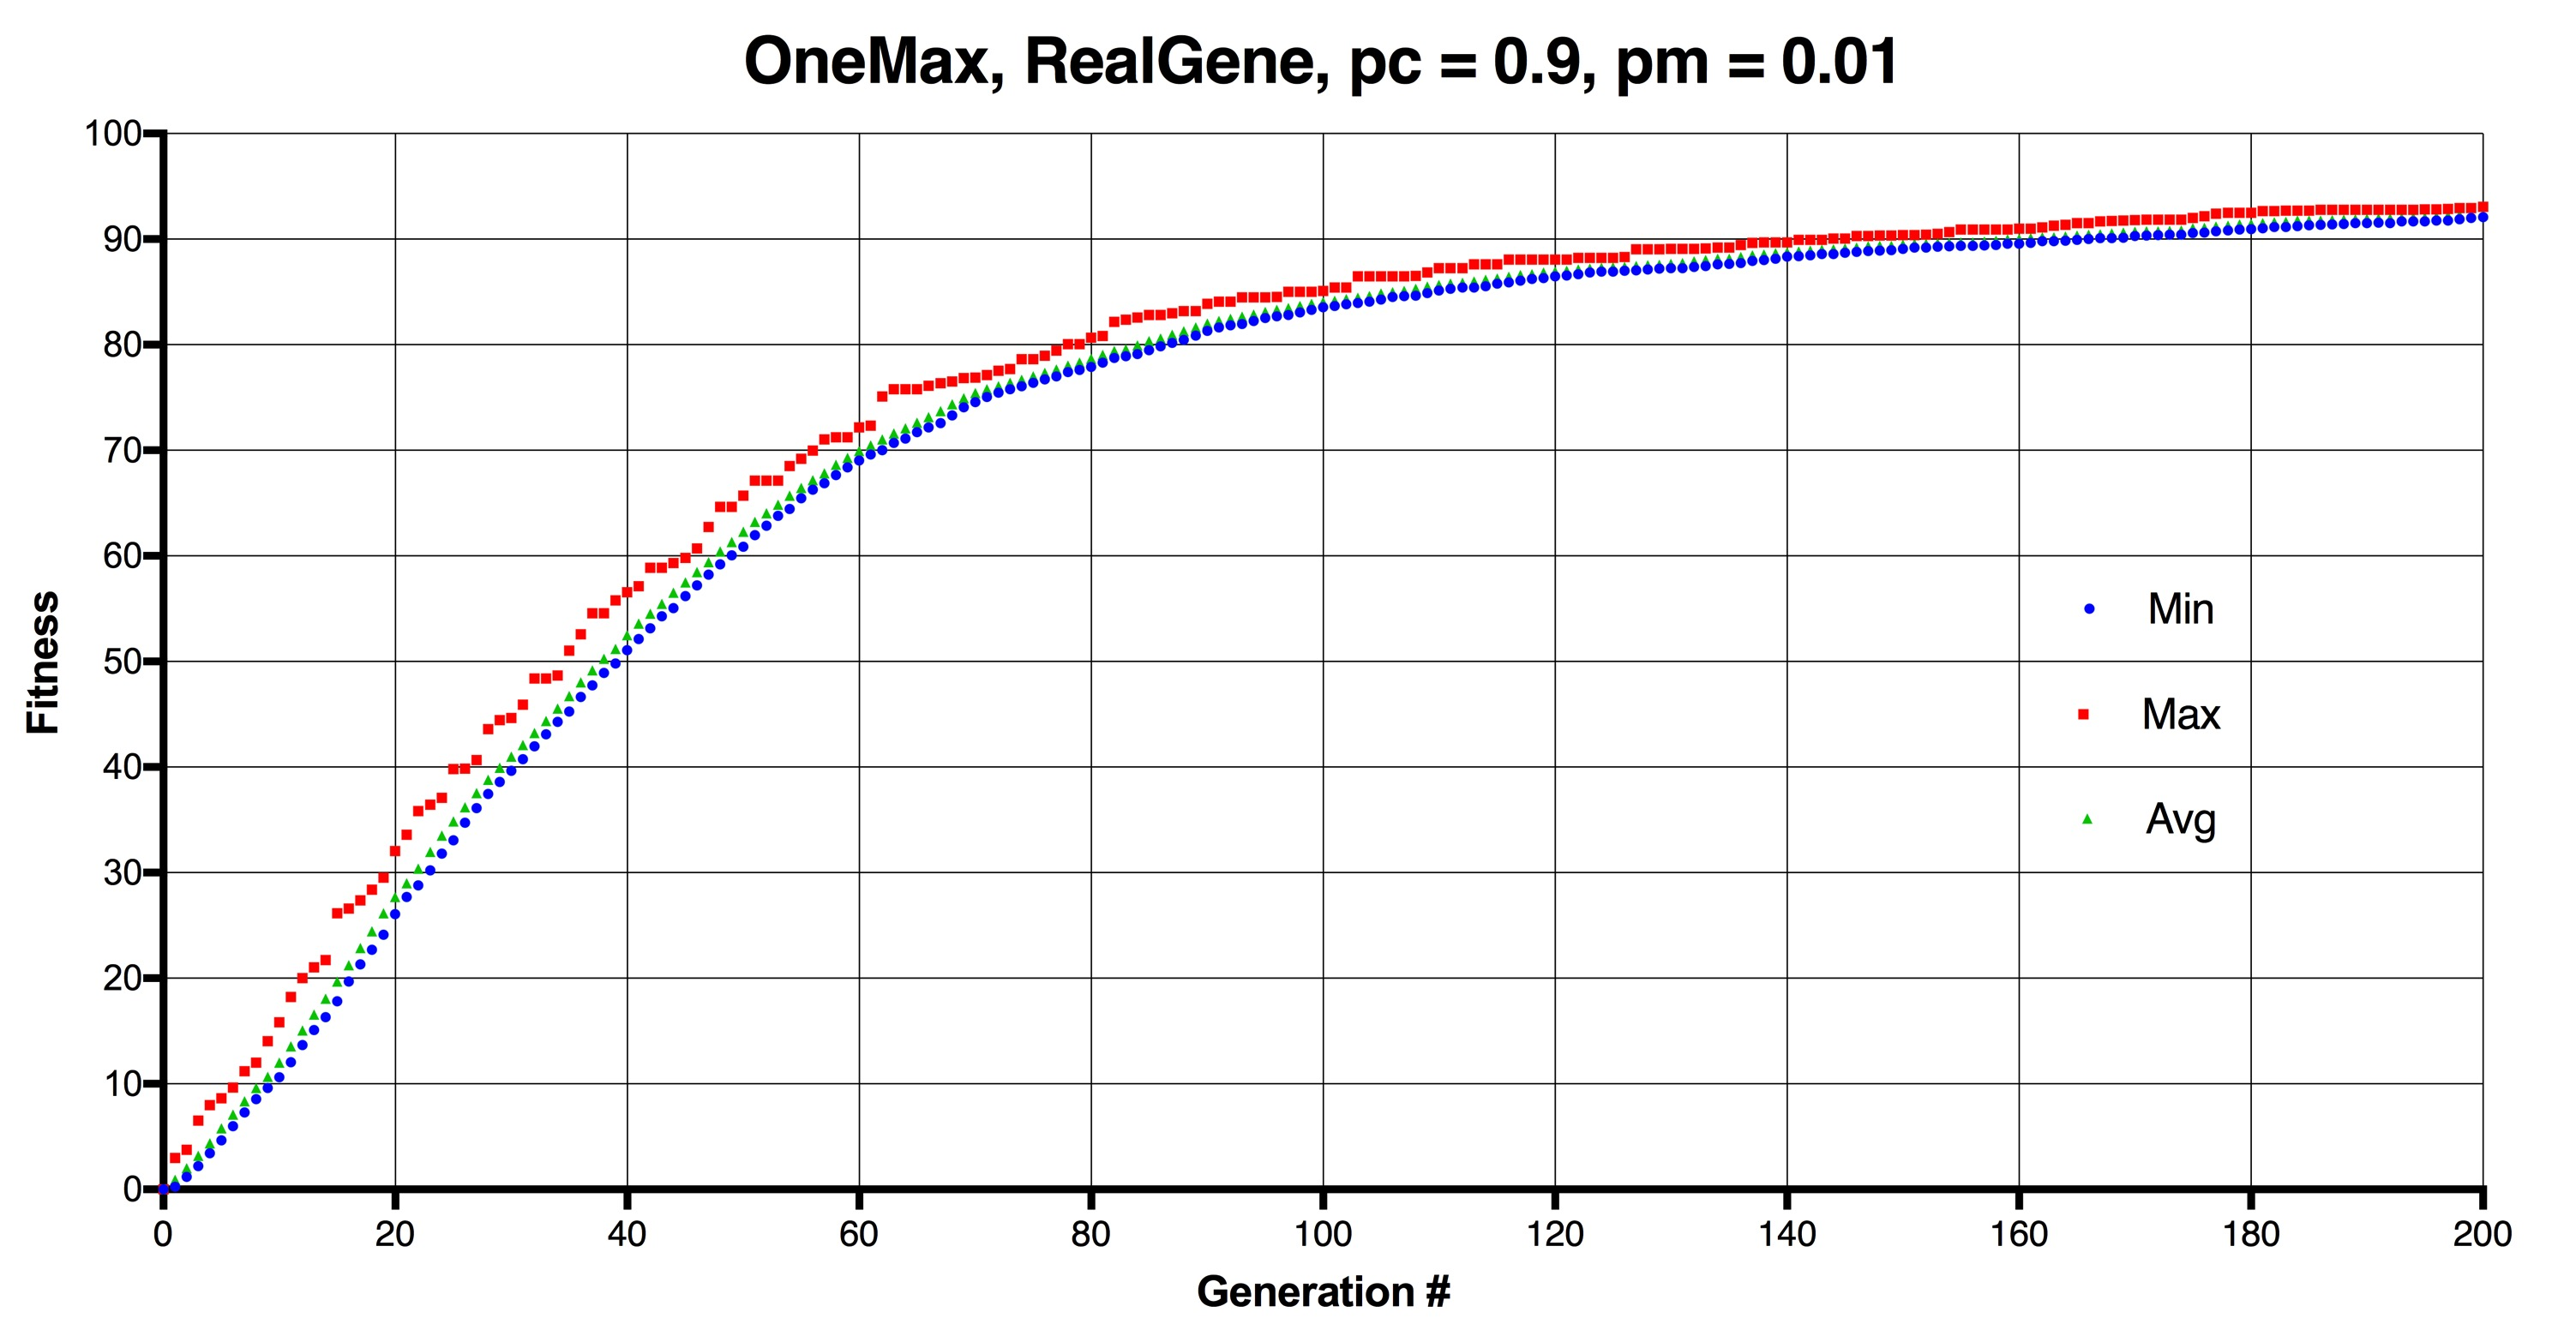
\includegraphics[width=1.0\textwidth]{onemax_real.jpg}
    \caption{Evolução do fitness para o problema do OneMax Real mostrando mínimo, máximo e valor médio ($p_c=0.9$, $p_m=0.01$).}
    \label{fig:onemax_real}
\end{figure}

Os pontos de qualquer uma das medições (média, mínimo e máximo) parecem formar uma curva. Descobri-la fugiu do escopo deste trabalho, mas tal formato pode estar associado à probabilidade de se aumentar a expressividade de um gene. Na execução deste AG, cada gene é levado para mutação com probabilidade $p_m$. Se um gene tiver uma expressividade $0 < x < 1$, a mutação (assumida uniforme) possui uma probabilidade $(1-x)$ de aumentá-la. Logo, a expressividade aumentará em uma dada geração com probabilidade:

\begin{equation}
	p_m(1-x)
\end{equation}

\subsection{Caso Adaptativo}

Os efeitos notados para o OneMax Booleano se repetiram aqui. Como se pode ver nas figuras \ref{fig:onemax_real_adaptive}, a população se estabilizou após cerca de 110 gerações, o que indica que a mutação se estabilizou em um determinado valor.

\begin{figure}[ht!]
    \centering 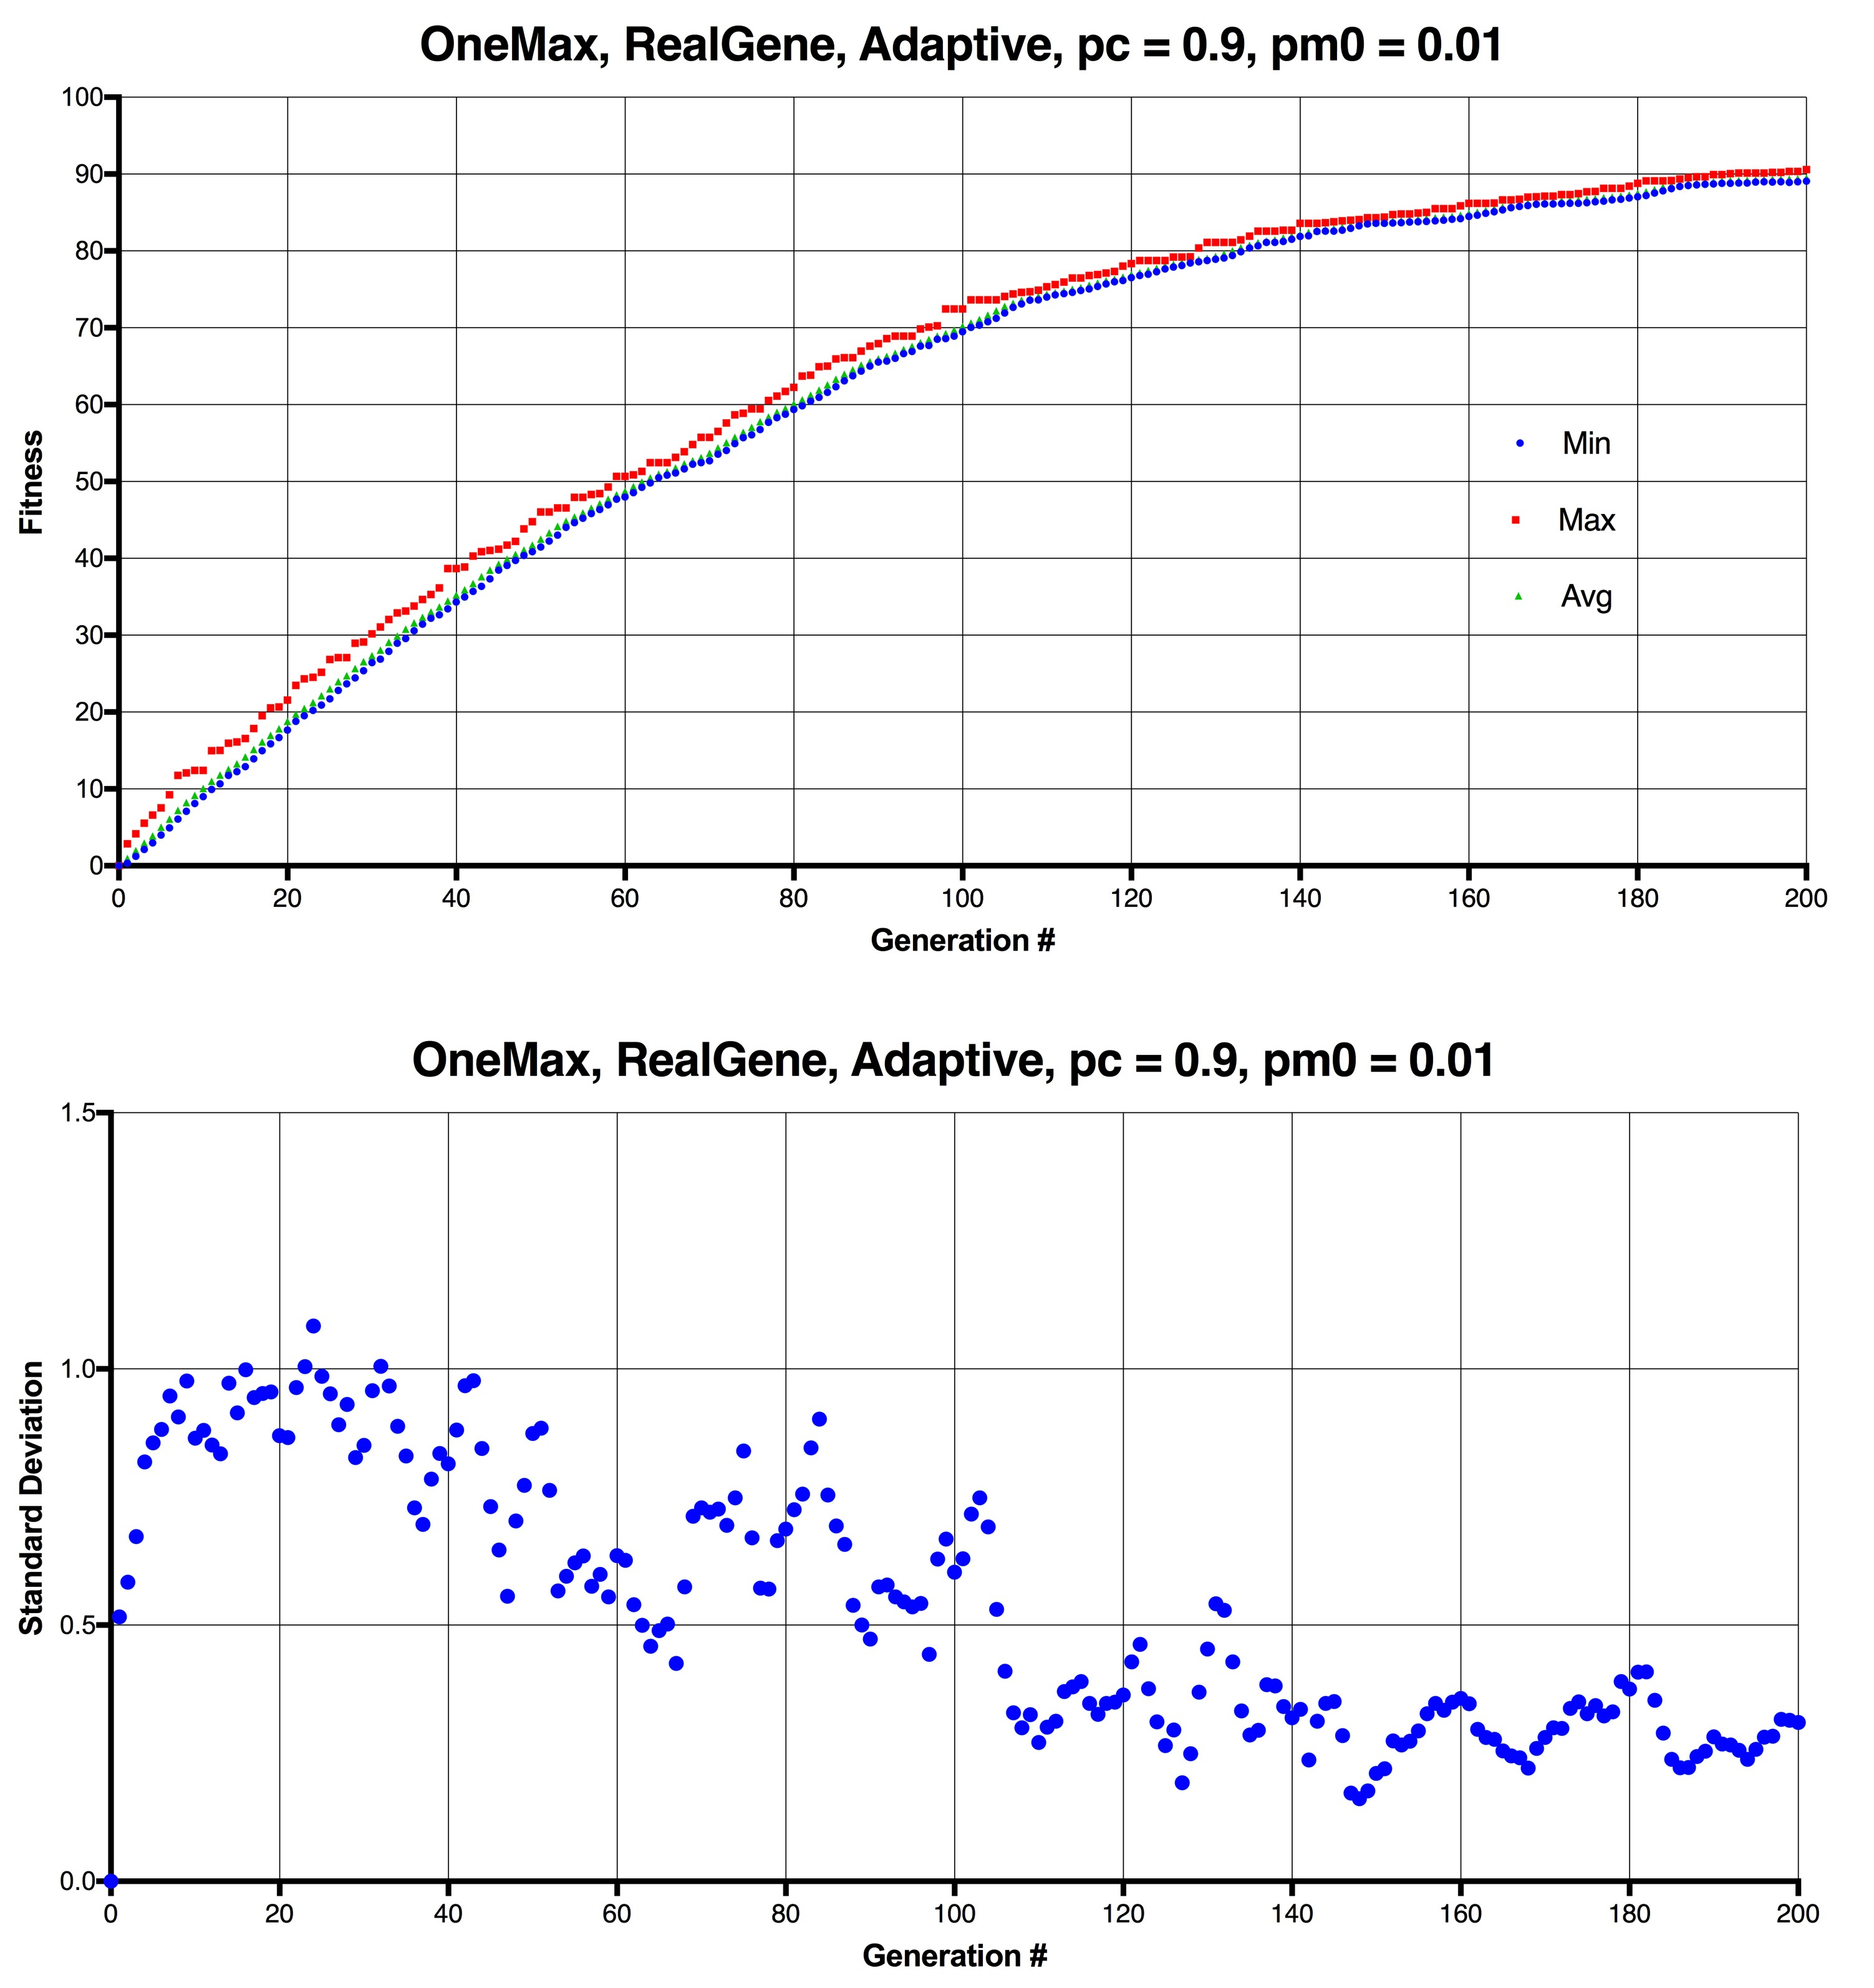
\includegraphics[width=1.0\textwidth]{onemax_real_adaptive.jpg}
    \caption{Evolução do fitness para o problema do OneMax Real Adaptativo mostrando mínimo, máximo e valor médio ($p_c=0.9$, ${p_m}_0=0.01$).}
    \label{fig:onemax_real_adaptive}
\end{figure}

Vemos também que o desvio padrão dos valores de fitness aparentou crescer ao longo das gerações. Isso se deu mais por conta do aumento de $p_m$ após 73 gerações, mostrado na figura \ref{fig:onemax_real_adaptive_pm}. Comparado ao OneMax Booleano, o $p_m$ atingiu valores maiores próximo às últimas gerações (oscilando em torno de 0.04), o que pode ter contribuído para o aumento do desvio padrão, mesmo com a média dos valores de fitness se mantendo relativamente no mesmo valor.

\begin{figure}[ht!]
    \centering 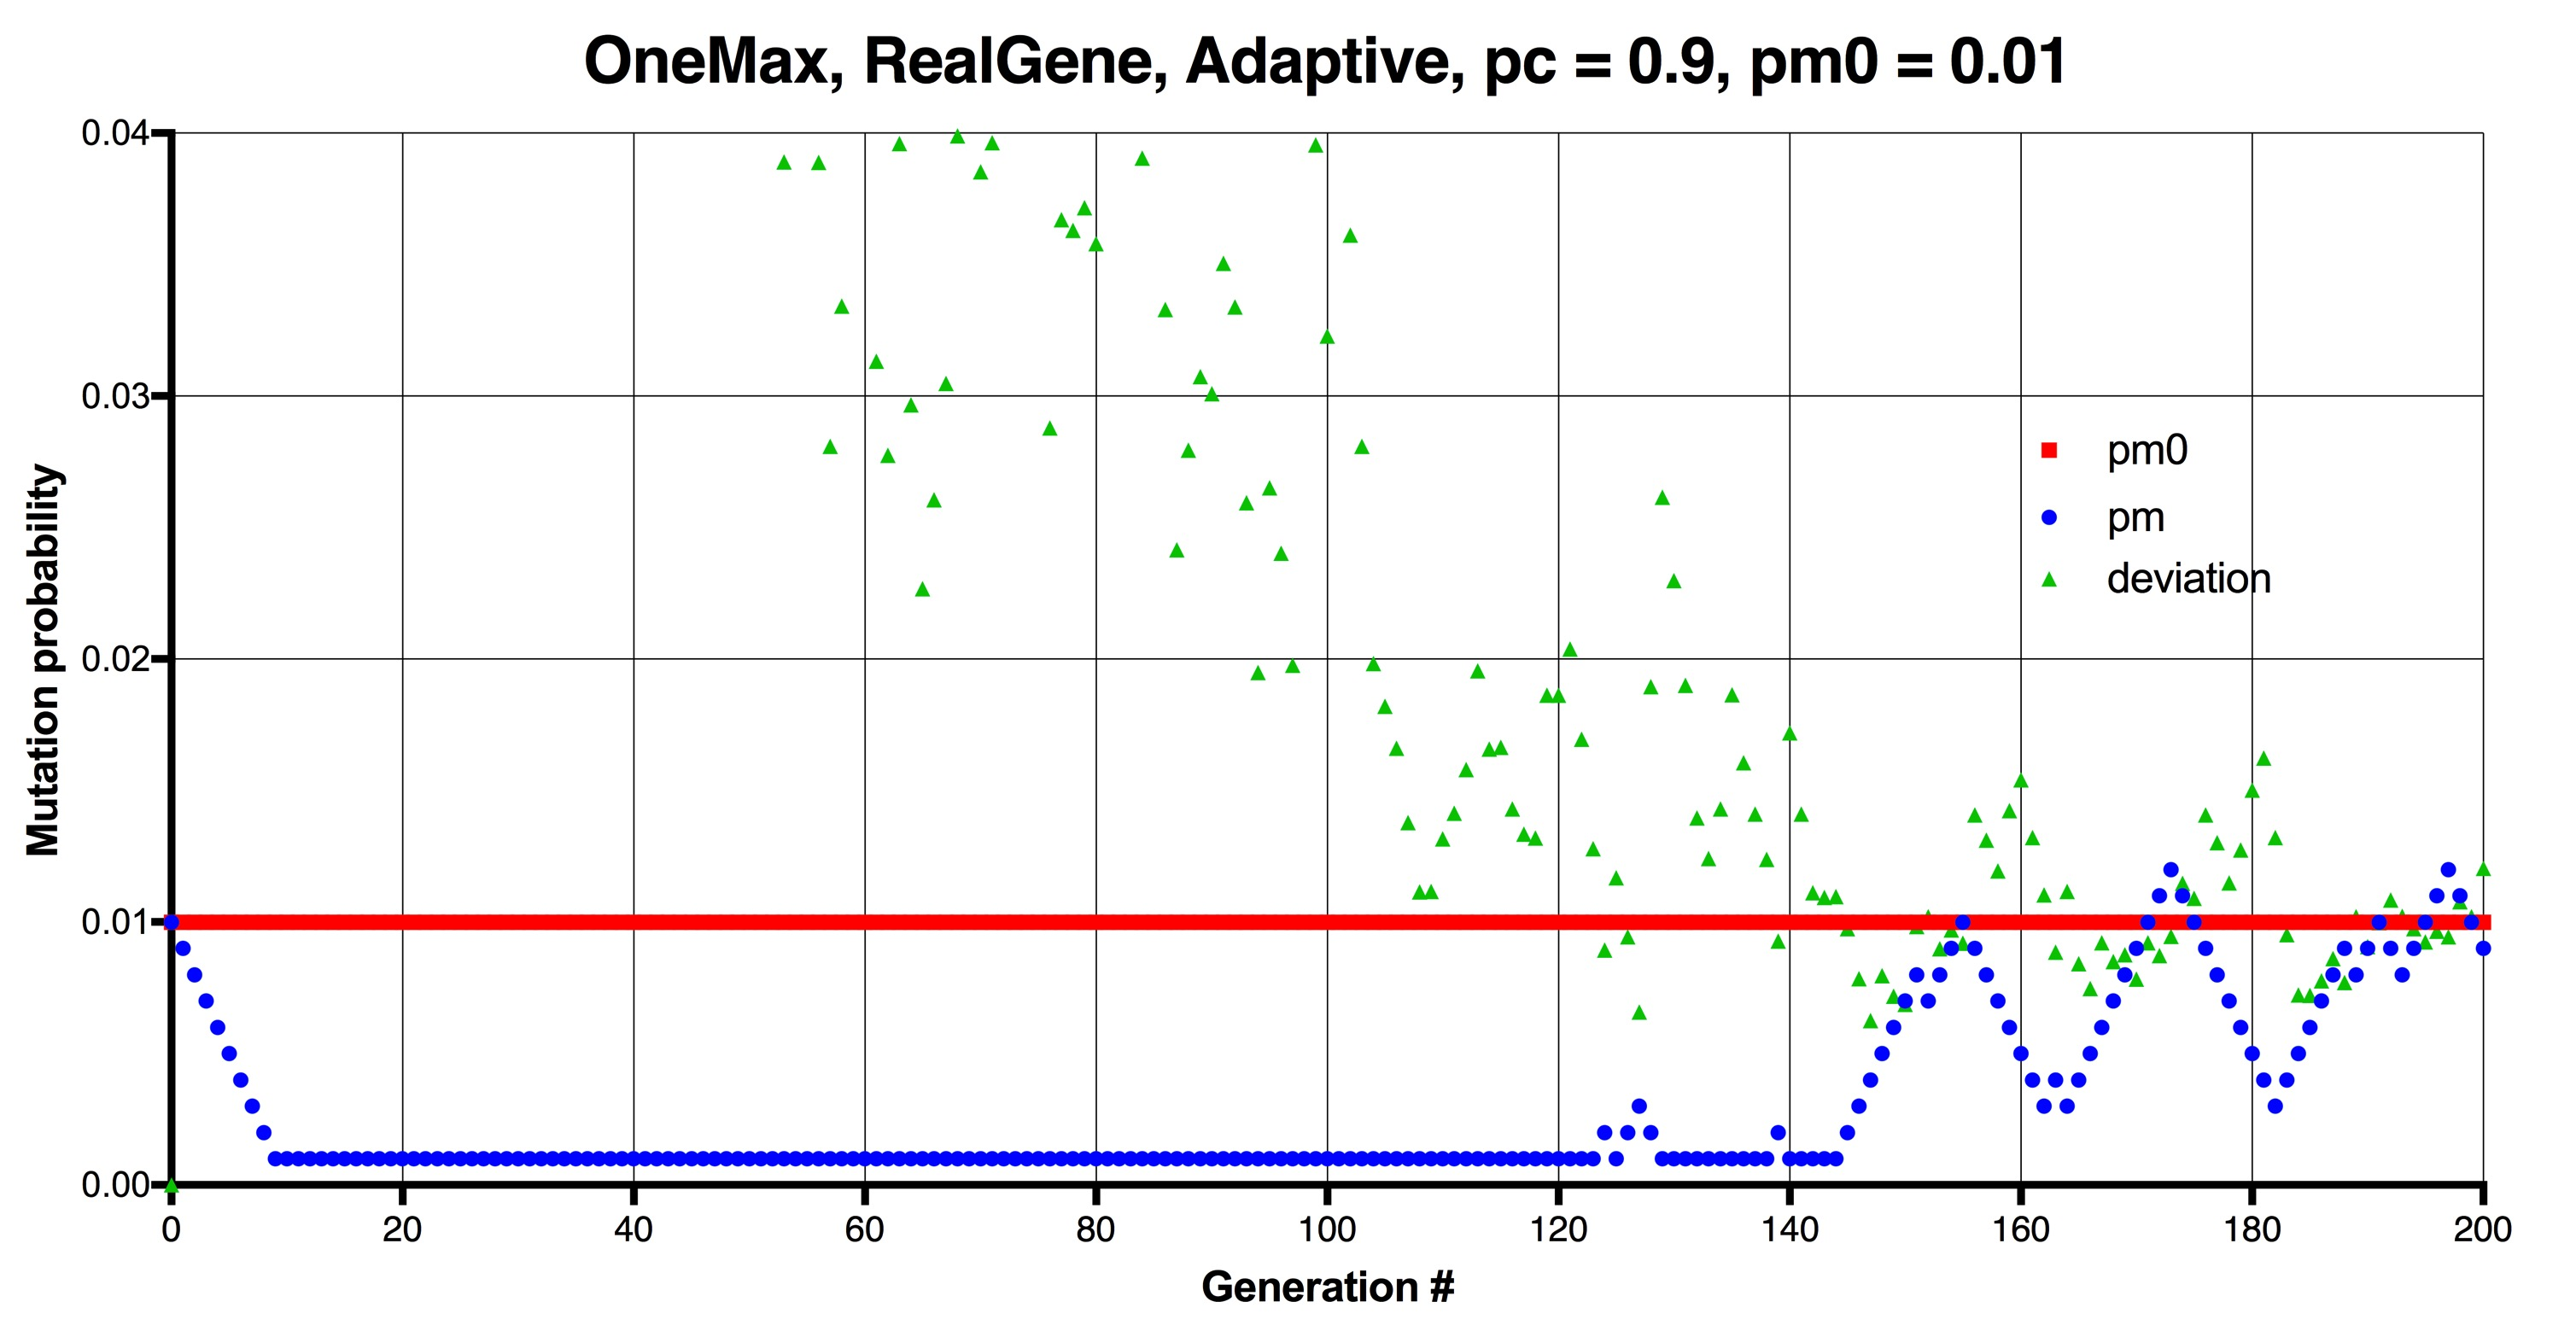
\includegraphics[width=1.0\textwidth]{onemax_real_adaptive_pm.jpg}
    \caption{Probabilidade de mutação ao longo das gerações para o problema do OneMax Real Adaptativo ($p_c=0.9$, ${p_m}_0=0.01$).}
    \label{fig:onemax_real_adaptive_pm}
\end{figure}

Os dados de interesse vindos destas simulações podem ser encontrados na tabela  \ref{tab:onemax_real}.

\begin{table}
\caption{Dados coletados do problema do OneMax Real ($p_m = 0.01$).}
\label{tab:onemax_real}

\center
\begin{tabular}{|c|cc|}
	\hline
	Algoritmo analisado (AG = caso estático) 	& AG		& AGA		\\
	\hline
	Fitness máximo após 100 gerações			& $85.115$	& $72.452$	\\
	Fitness médio após 100 gerações				& $84.048$	& $70.186$	\\
	Fitness máximo após 200 gerações 			& $93.083$	& $90.585$	\\
	Fitness médio após 200 gerações 			& $92.355$	& $89.507$	\\
	Valor final de $p_m$						& $0.01$ 	& $0.009$	\\
	Valor mínimo de $p_m$						& $0.01$	& $0.001$	\\
	Valor máximo de $p_m$						& $0.01$	& $0.012$	\\
	Valor médio de $p_m$						& $0.01$	& $0.00300$	\\
	Valor médio de $p_m$ (últimas 100 gerações)	& $0.01$	& $0.00458$	\\
	\hline
\end{tabular}
\end{table}

\section{Caixeiro Viajante Adaptado}

Para as simulações deste problema, utilizou-se então o grafo do programa Open-Source DEAP com 17 cidades \cite{DEAP_JMLR2012, deap2016tsp}. Tal grafo é conexo, completo e bidirecionado, e sua distância mínima (começando na primeira cidade) é 2085. Ele está presente na listagem \ref{lst:cidades}.

\begin{lstlisting}[float, floatplacement=H, caption={Mapa de cidades para o problema do Caixeiro Viajante Adaptado.}, label=lst:cidades]
[0, 633, 257, 91, 412, 150, 80, 134, 259, 505, 353, 324, 70, 211, 268, 246, 121],
[633, 0, 390, 661, 227, 488, 572, 530, 555, 289, 282, 638, 567, 466, 420, 745, 518],
[257, 390, 0, 228, 169, 112, 196, 154, 372, 262, 110, 437, 191, 74, 53, 472, 142],
[91, 661, 228, 0, 383, 120, 77, 105, 175, 476, 324, 240, 27, 182, 239, 237, 84],
[412, 227, 169, 383, 0, 267, 351, 309, 338, 196, 61, 421, 346, 243, 199, 528, 297],
[150, 488, 112, 120, 267, 0, 63, 34, 264, 360, 208, 329, 83, 105, 123, 364, 35],
[80, 572, 196, 77, 351, 63, 0, 29, 232, 444, 292, 297, 47, 150, 207, 332, 29],
[134, 530, 154, 105, 309, 34, 29, 0, 249, 402, 250, 314, 68, 108, 165, 349, 36],
[259, 555, 372, 175, 338, 264, 232, 249, 0, 495, 352, 95, 189, 326, 383, 202, 236],
[505, 289, 262, 476, 196, 360, 444, 402, 495, 0, 154, 578, 439, 336, 240, 685, 390],
[353, 282, 110, 324, 61, 208, 292, 250, 352, 154, 0, 435, 287, 184, 140, 542, 238],
[324, 638, 437, 240, 421, 329, 297, 314, 95, 578, 435, 0, 254, 391, 448, 157, 301],
[70, 567, 191, 27, 346, 83, 47, 68, 189, 439, 287, 254, 0, 145, 202, 289, 55],
[211, 466, 74, 182, 243, 105, 150, 108, 326, 336, 184, 391, 145, 0, 57, 426, 96],
[268, 420, 53, 239, 199, 123, 207, 165, 383, 240, 140, 448, 202, 57, 0, 483, 153],
[246, 745, 472, 237, 528, 364, 332, 349, 202, 685, 542, 157, 289, 426, 483, 0, 336],
[121, 518, 142, 84, 297, 35, 29, 36, 236, 390, 238, 301, 55, 96, 153, 336, 0]
\end{lstlisting}

\subsection{Caso Estático ($p_m = 0.01$)}

Para o caso estático com $p_m = 0.01$, mostrado na figura \ref{fig:tsp001}, vemos que este valor de $p_m$ incentiva pouco o encontro de soluções melhores, demonstrado pela melhor solução (pontos azuis) ter mantido o mesmo valor por mais de 100 gerações. Em termos de desvio padrão, percebeu-se que $p_m = 0.01$ foi capaz apenas de igualar os valores de fitness de modo rápido (uma vez que há apenas 15 genes a serem recombinados).

\begin{figure}[ht!]
    \centering 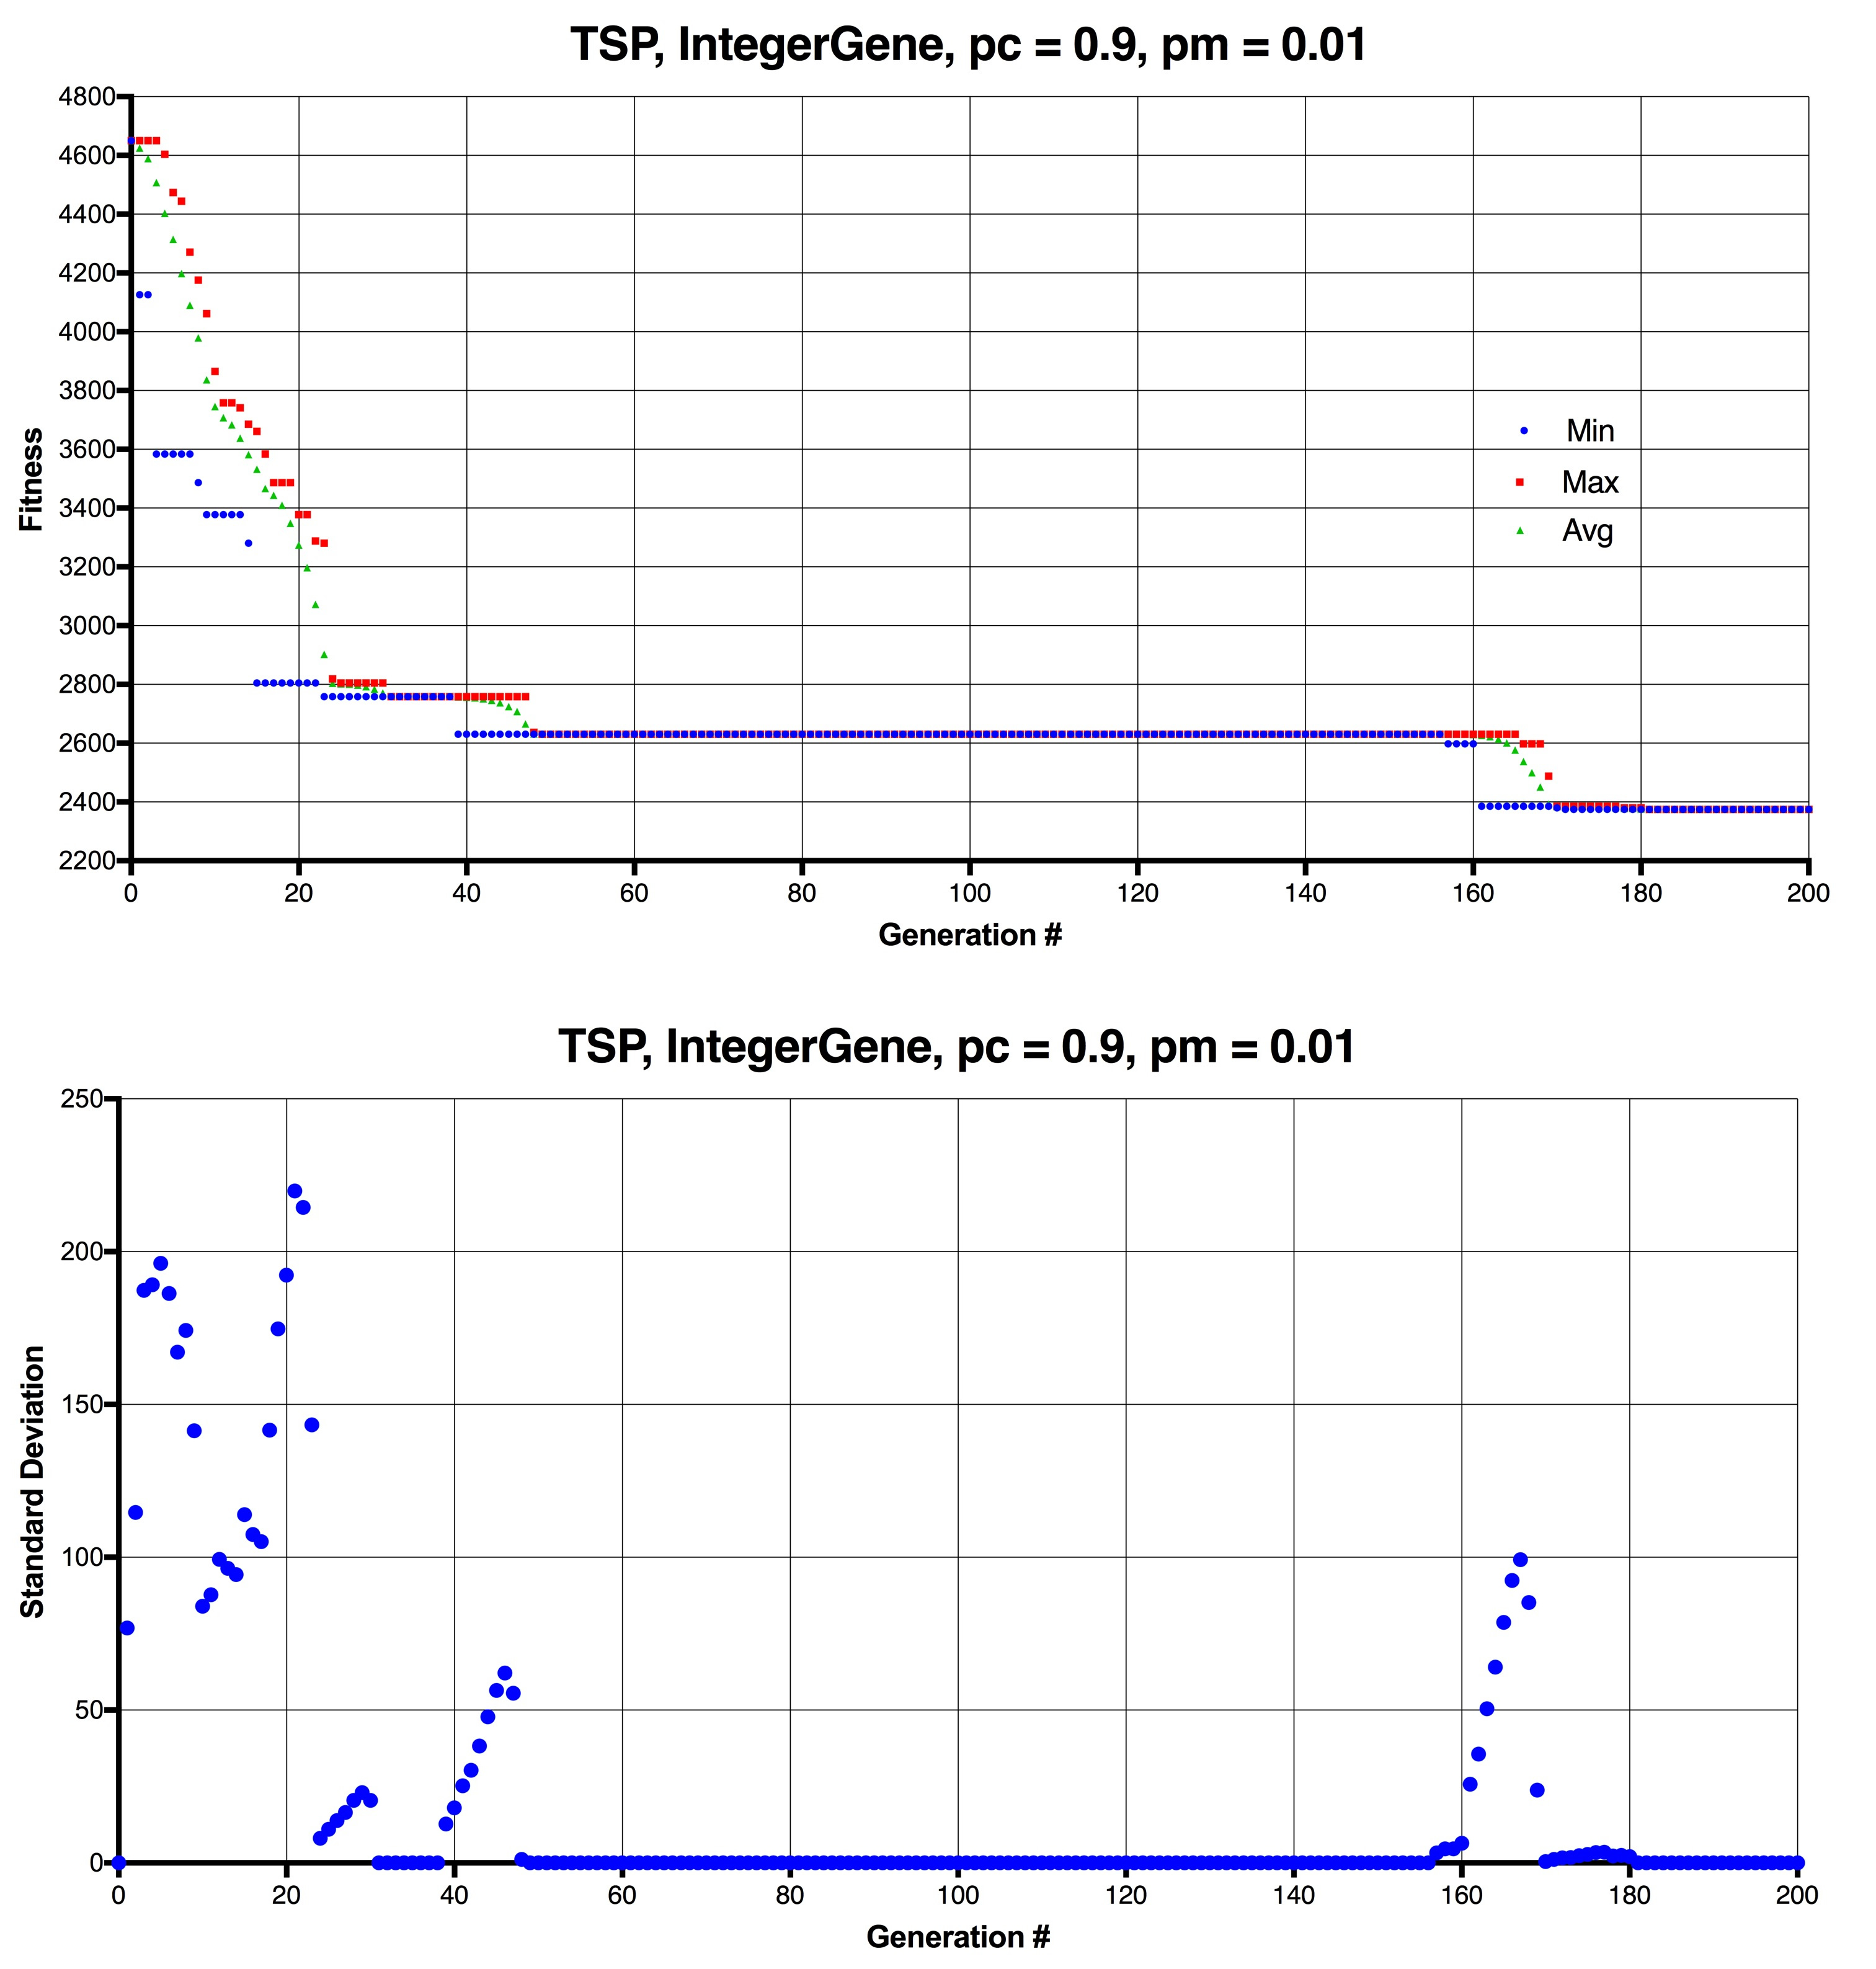
\includegraphics[width=1.0\textwidth]{tsp_001.jpg}
    \caption{Evolução do fitness para o problema do Caixeiro Viajante Adaptado mostrando mínimo, máximo, valor médio e desvio padrão ($p_c=0.9$, $p_m=0.01$). O menor caminho encontrado tem distância total de 2375.}
    \label{fig:tsp001}
\end{figure}

Uma possível interpretação foi a de que o AG travou em um mínimo local, e um valor maior de $p_m$ poderia resolver este problema. Optou-se então por testar $p_m = 0.2$.

\subsection{Caso Estático ($p_m = 0.2$)}

Para o caso estático com $p_m = 0.2$, mostrado na figura \ref{fig:tsp02}, vemos que $p_m = 0.2$ conseguiu chegar a uma solução melhor (2300 contra 2375). No entanto, o comportamento do valor mínimo de fitness ainda foi muito próximo daquele visto para $p_m = 0.01$ (agora mantendo a melhor solução por mais de 120 gerações). 

\begin{figure}[ht!]
    \centering 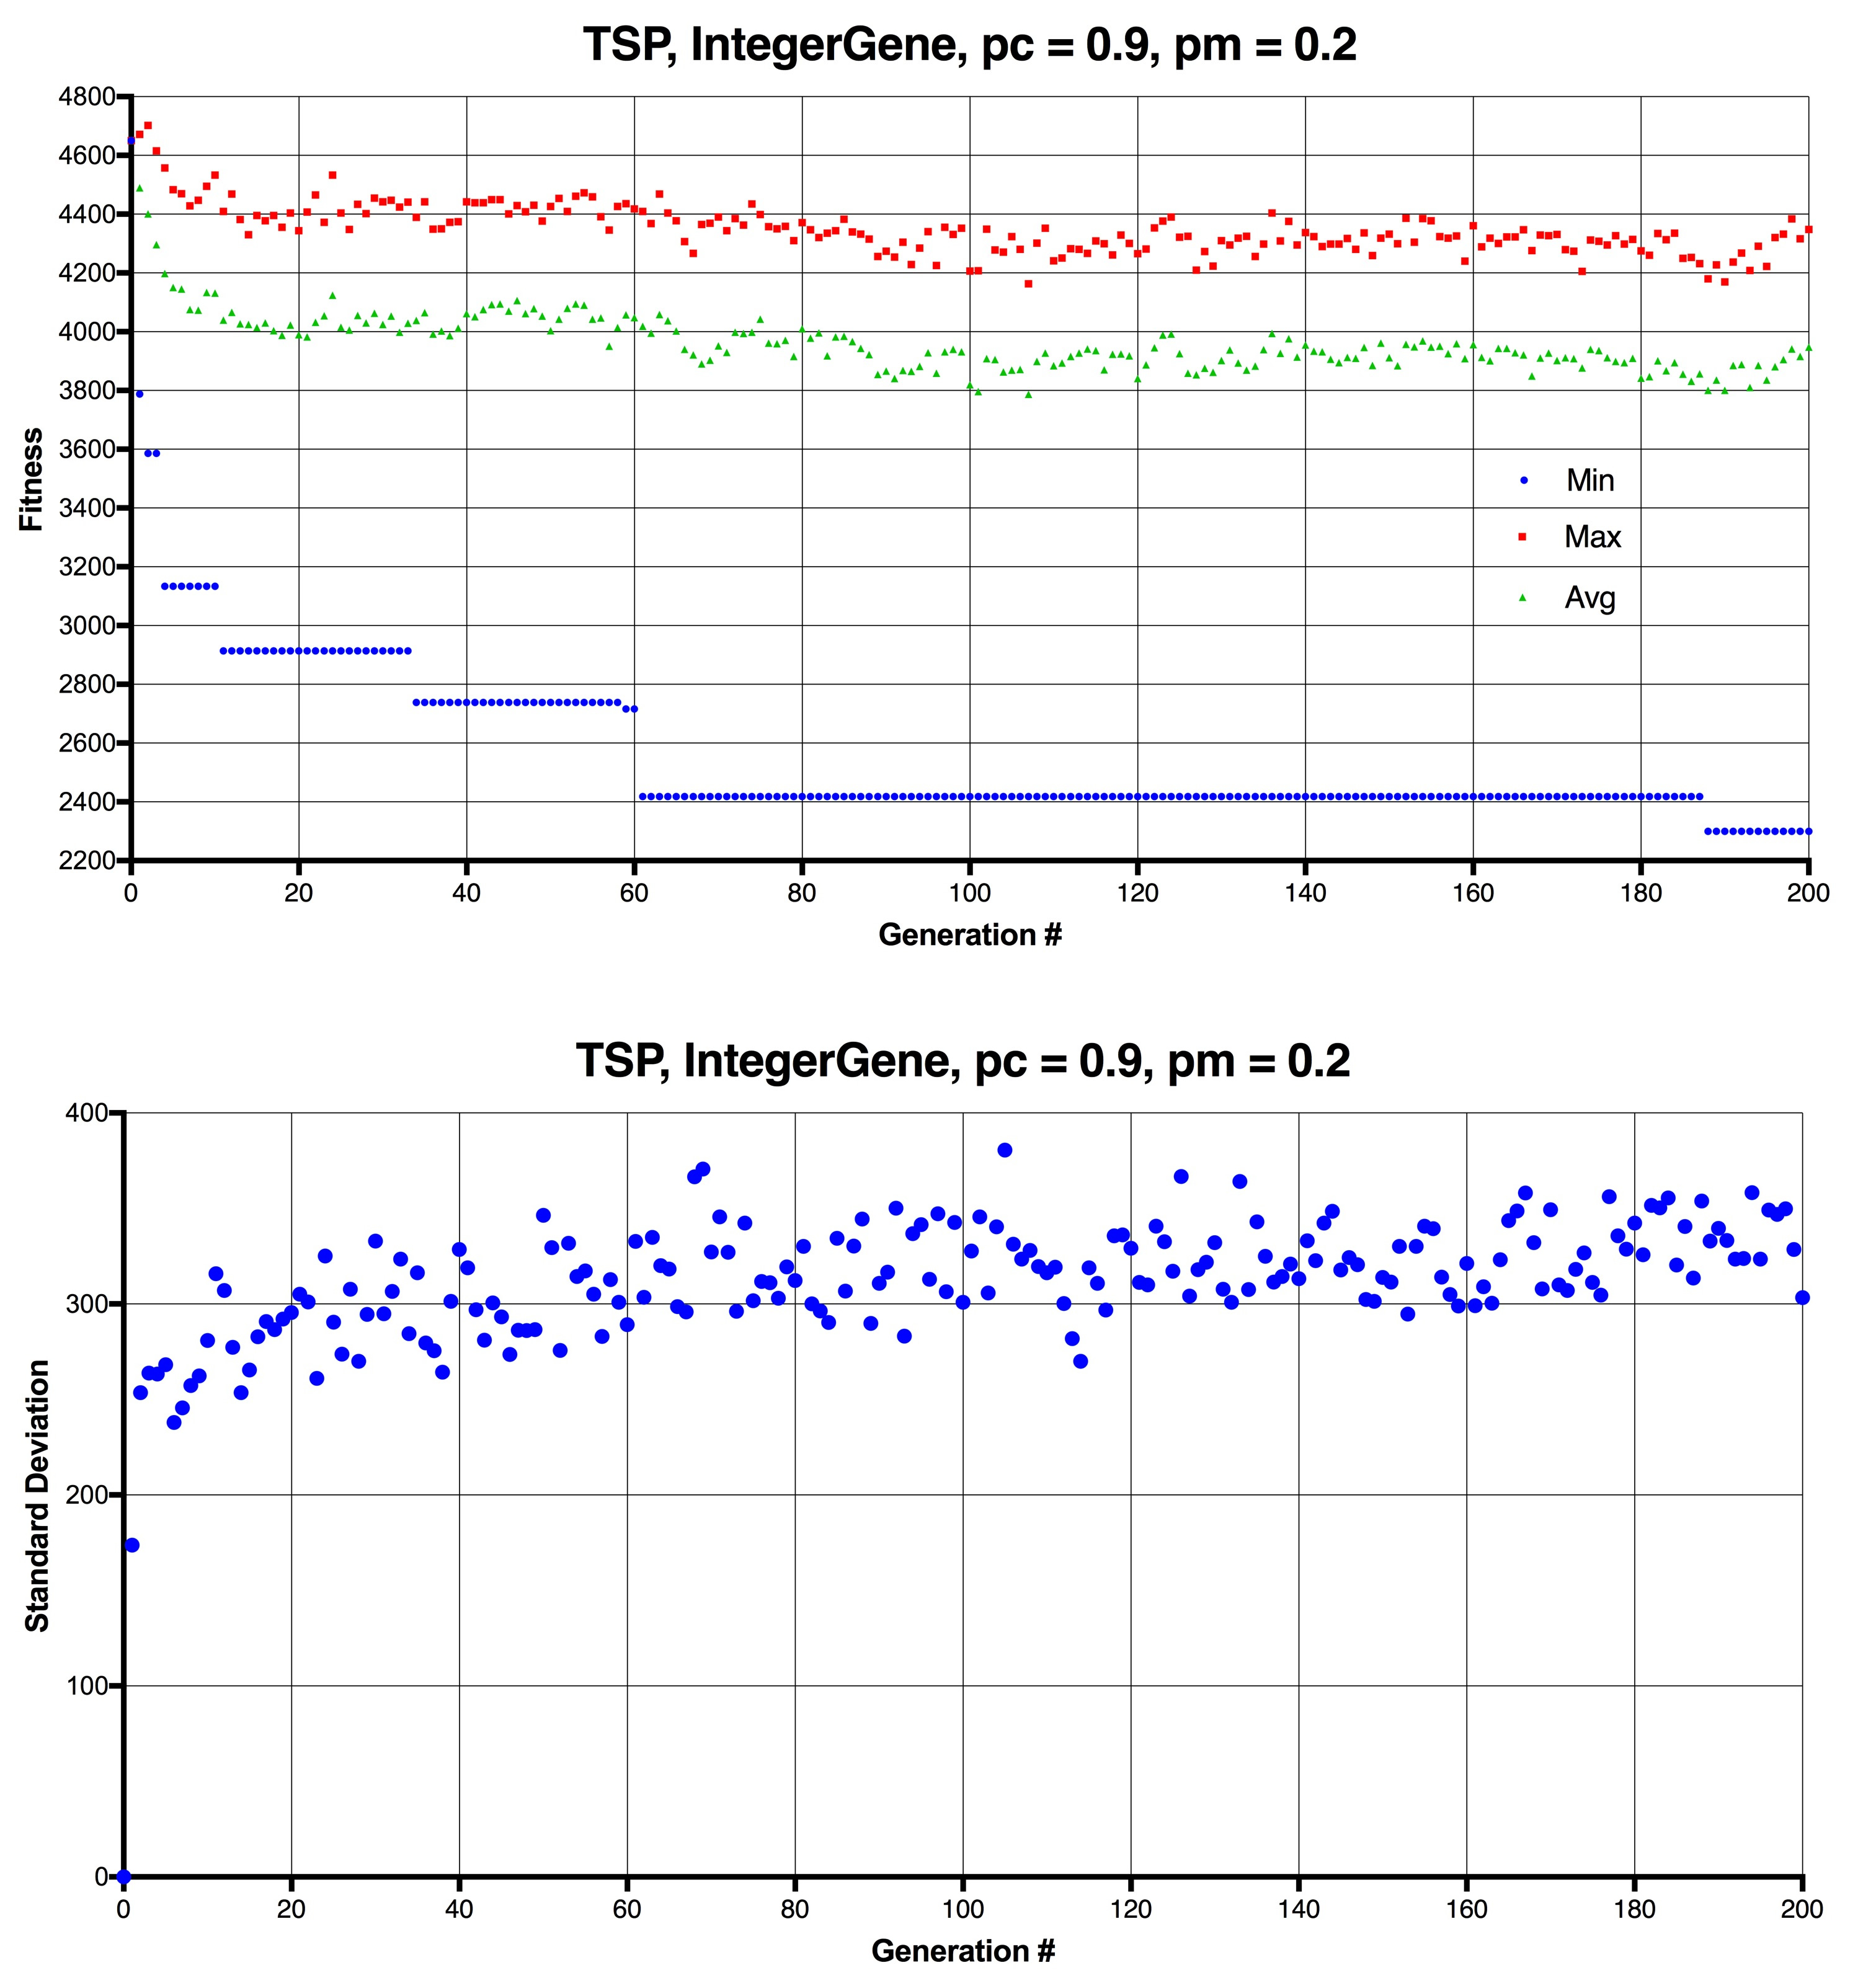
\includegraphics[width=1.0\textwidth]{tsp_02.jpg}
    \caption{Evolução do fitness para o problema do Caixeiro Viajante Adaptado mostrando mínimo, máximo, valor médio e desvio padrão ($p_c=0.9$, $p_m=0.2$). O menor caminho encontrado tem distância total de 2300.}
    \label{fig:tsp02}
\end{figure}

O desvio padrão mostrou que uma mutação mais intensa incentiva o surgimento de muito mais soluções. No entanto, tais soluções são igualmente imprevisíveis aos olhos do problema, o que fez crer que aumentar $p_m$ (para 20\%, que já é absurdamente alto) não fez diferença para o caso estático.

\subsection{Caso Adaptativo ($p_m = 0.01$)}

O caso adaptativo para $p_m = 0.01$ mostrou uma evolução bem diferente do caso estático. Como visto na figura \ref{fig:tsp_001_adaptative}, os indivíduos também conseguiram igualar seus valores de fitness de modo relativamente rápido, mas a melhor solução pôde mudar bem mais rápido. A melhor solução ficou travada por não mais que 76 gerações (região azul entre as gerações 80 e 140), e mesmo assim, os demais indivíduos foram capazes de variar nesse intervalo, o que parece ter ajudado no encontro de soluções melhores. Tal comportamento das soluções pode ser observado também nos desvios padrões.

\begin{figure}[ht!]
    \centering 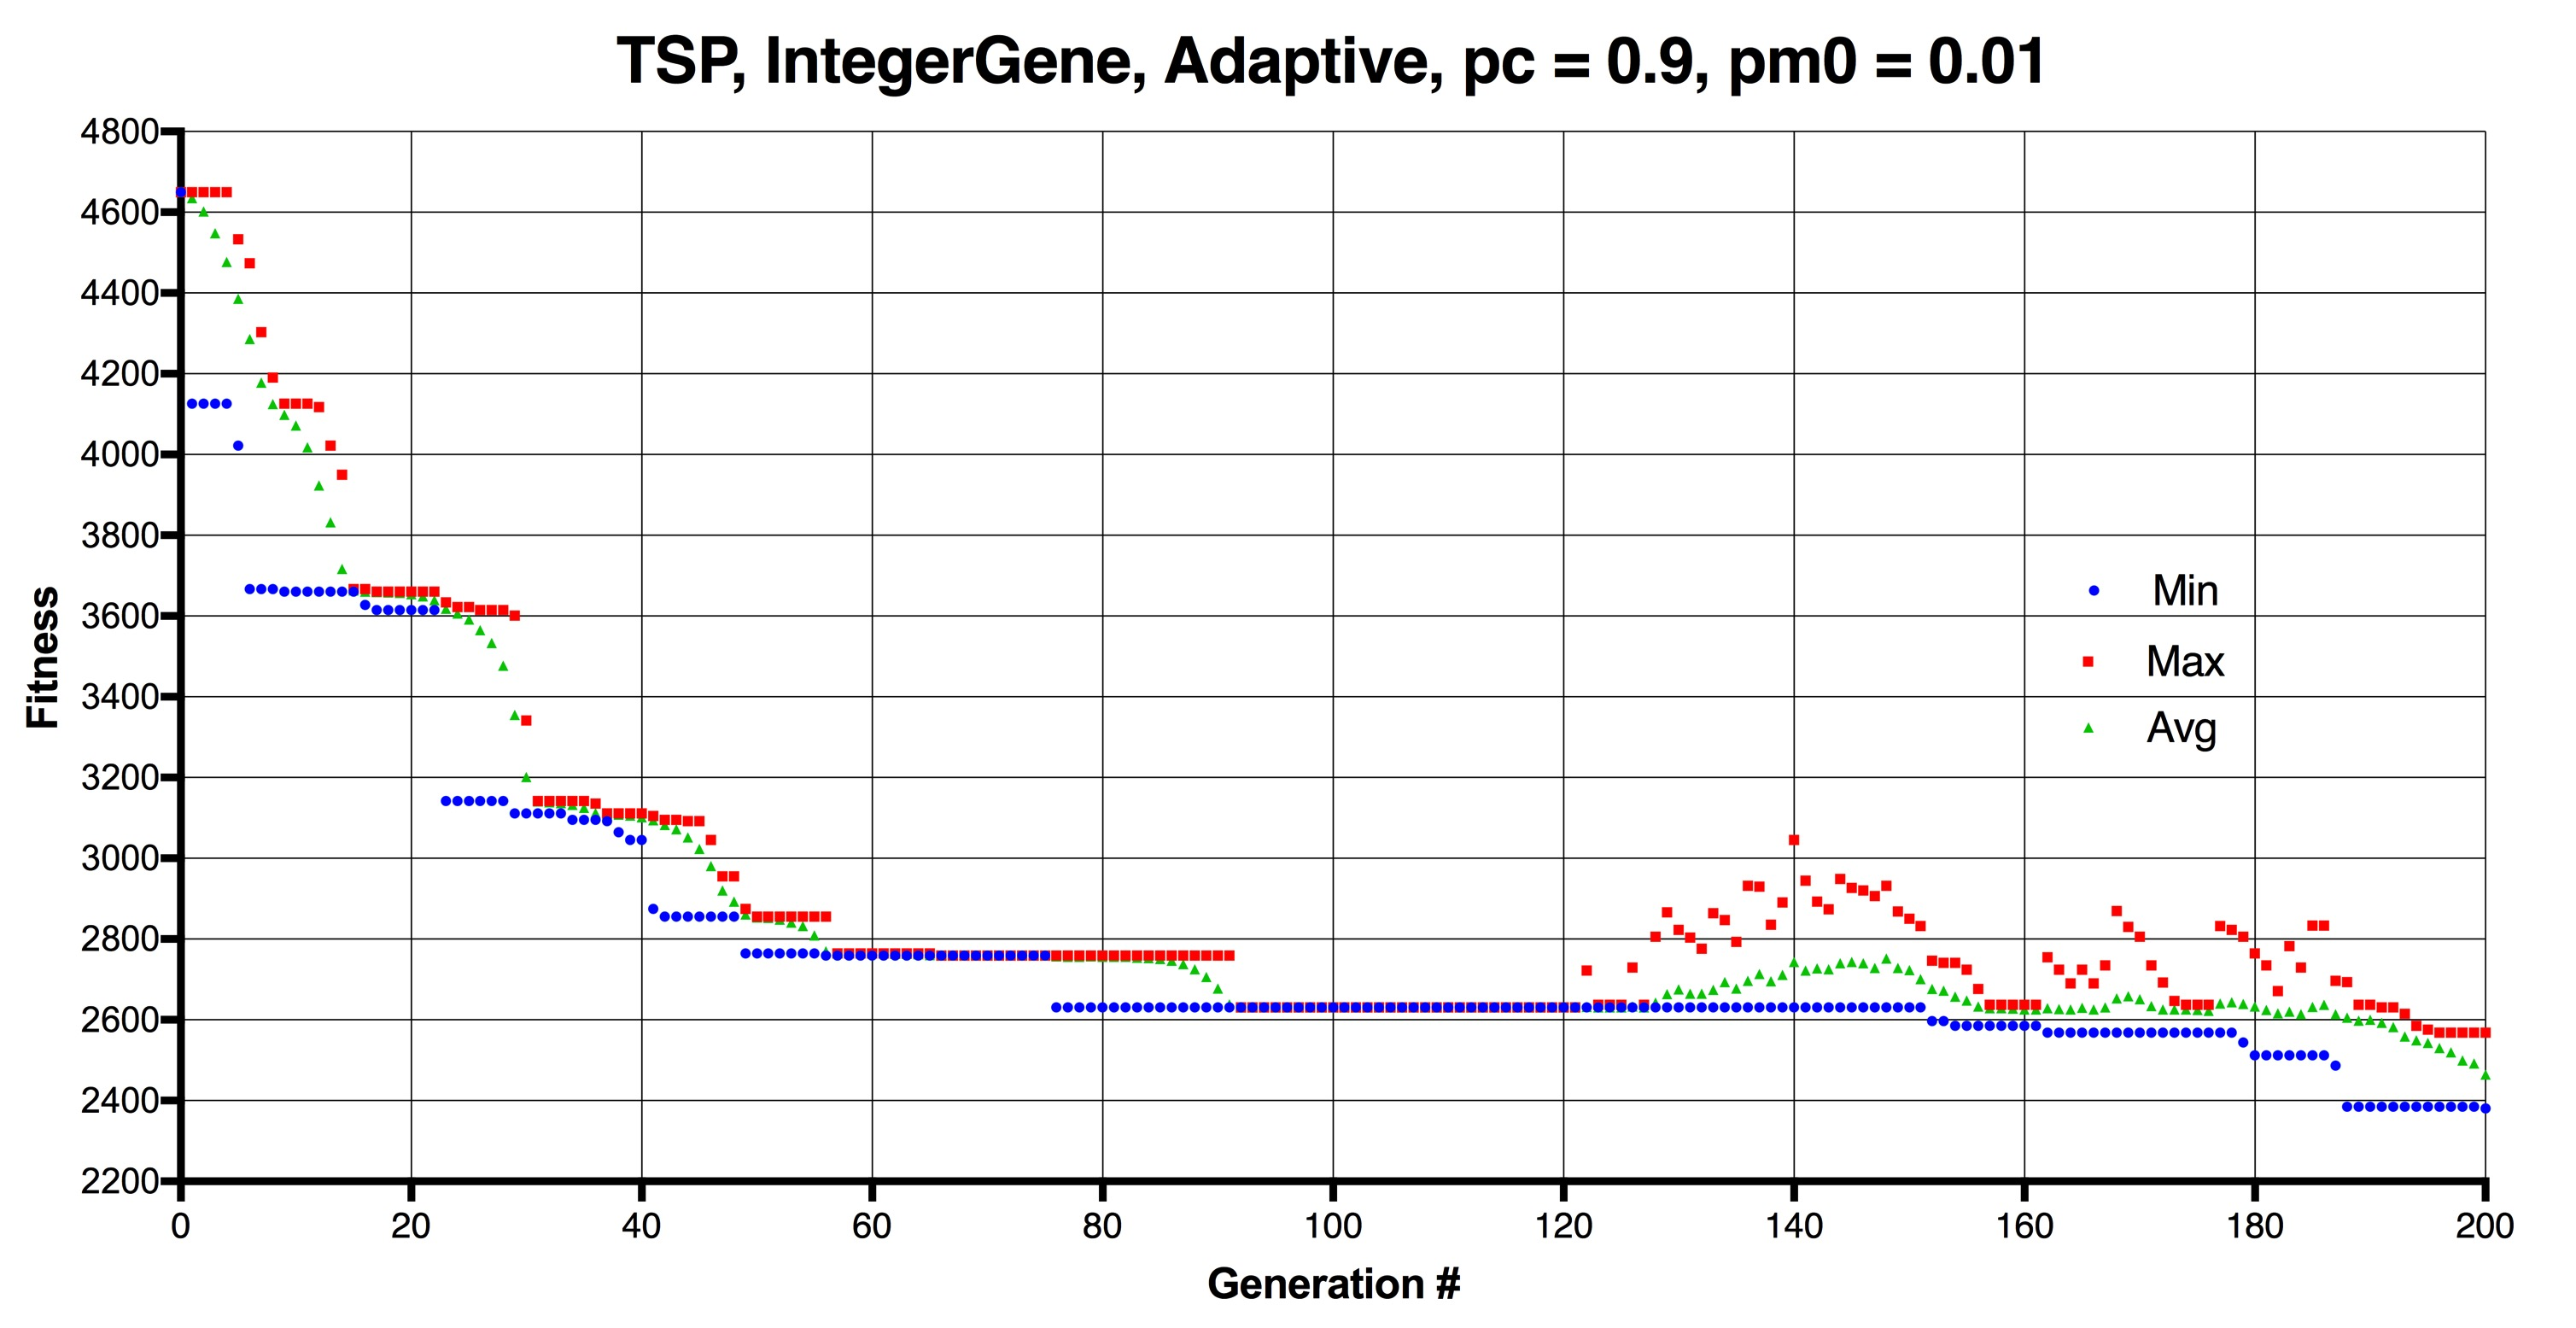
\includegraphics[width=1.0\textwidth]{tsp_001_adaptive.jpg}
    \caption{Evolução do fitness para o problema do Caixeiro Viajante Adaptado Adaptativo, mostrando mínimo, máximo, valor médio e desvio padrão ($p_c=0.9$, ${p_m}_0=0.01$). O menor caminho encontrado tem distância total de 2381.}
    \label{fig:tsp_001_adaptative}
\end{figure}

O funcionamento do AGA ficou bem mais evidente na figura \ref{fig:tsp_001_adaptive_pm}, com momentos de aumento e de redução de $p_m$ alternados com maior frequência. Fora isso, ${p_m}_0$ convergiu para um valor bem menor no final da execução (0.024). No entanto, ao contrário dos problemas OneMax, $p_m$ oscilou bastante também ao final das 200 gerações. Isso nos leva a crer que $0.01$ talvez não seja o melhor valor para inicializar ${p_m}_0$. Similar ao caso estático, simulou-se também ${p_m}_0 = 0.2$.

\begin{figure}[ht!]
    \centering 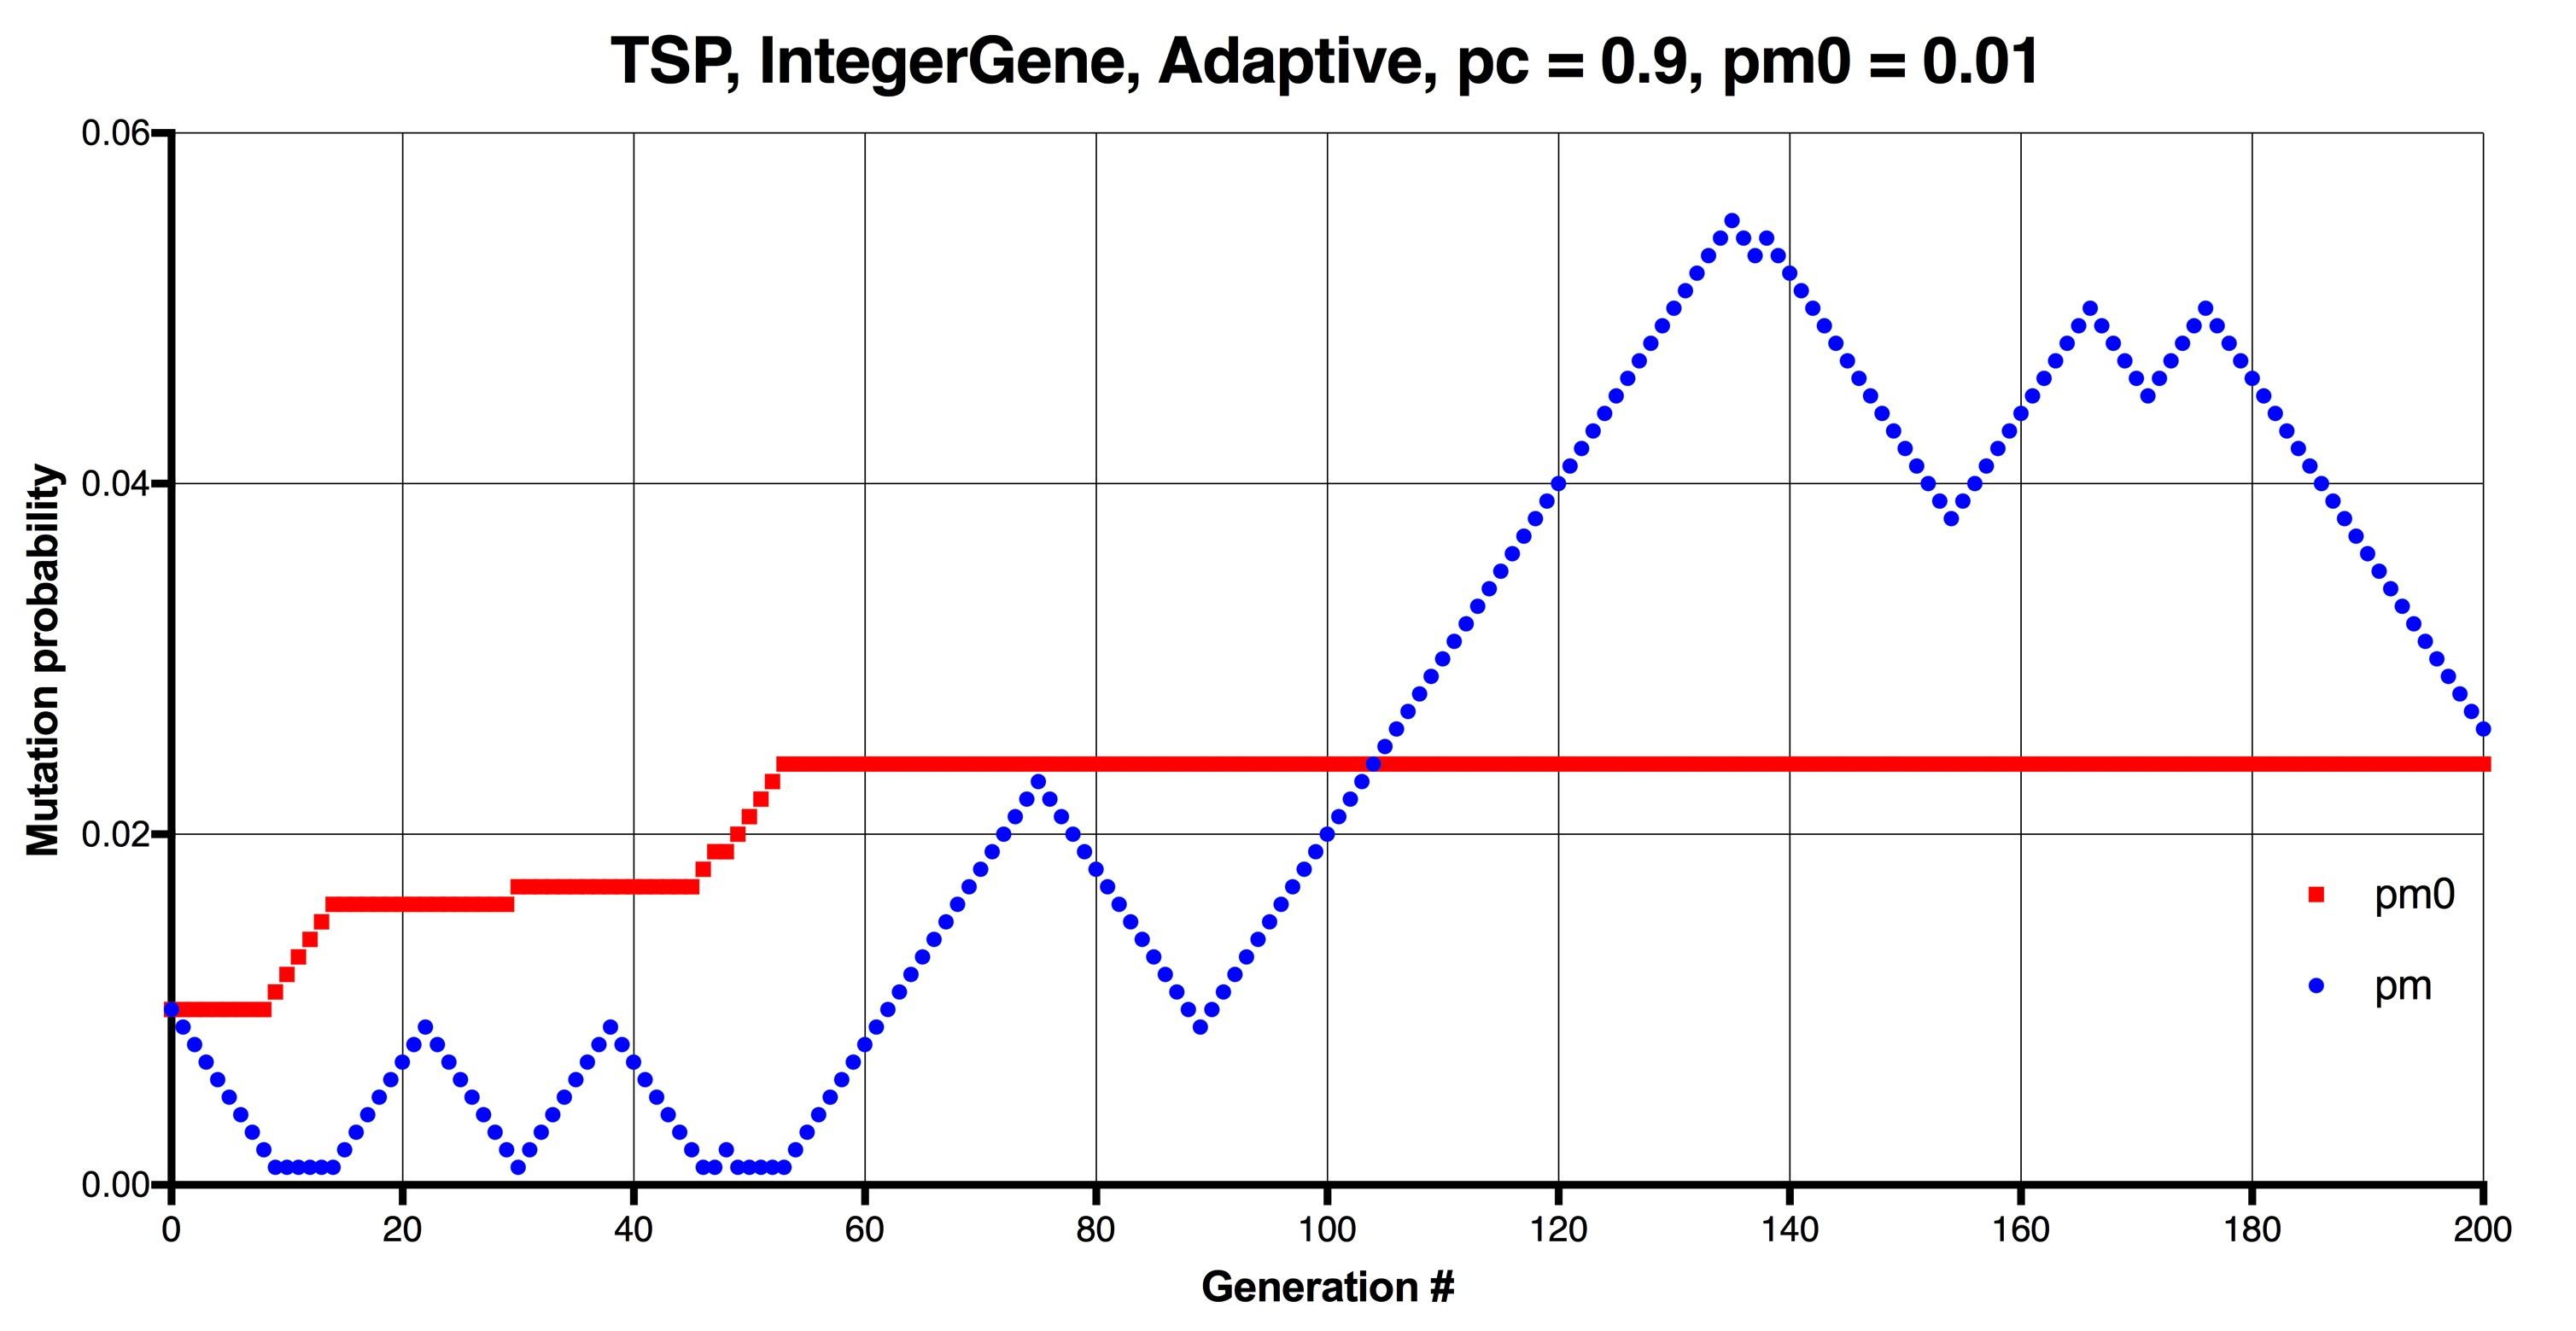
\includegraphics[width=1.0\textwidth]{tsp_001_adaptive_pm.jpg}
    \caption{Probabilidade de mutação ao longo das gerações para o problema do Caixeiro Viajante Adaptado Adaptativo ($p_c=0.9$, ${p_m}_0=0.01$).}
    \label{fig:tsp_001_adaptive_pm}
\end{figure}

\subsection{Caso Adaptativo ($p_m = 0.2$)}

O gráfico da figura \ref{fig:tsp_02_adaptative} encontrou o menor percurso dentre as simulações feitas aqui (2160). Não só isso, as melhores soluções pareceram ficar travadas por bem menos tempo (o pior caso, próximo do final da simulação, durou 34 gerações). Um outro efeito interessante também aconteceu: todas as curvas (mínimo, máximo e média) evoluíram de formas semelhantes, mesmo com uma mutação inicial intensa. Isso deu para observar também na evolução do desvio padrão, que conseguiu diminuir com o tempo e ficar mais ou menos estável ao longo das gerações.

\begin{figure}[ht!]
    \centering 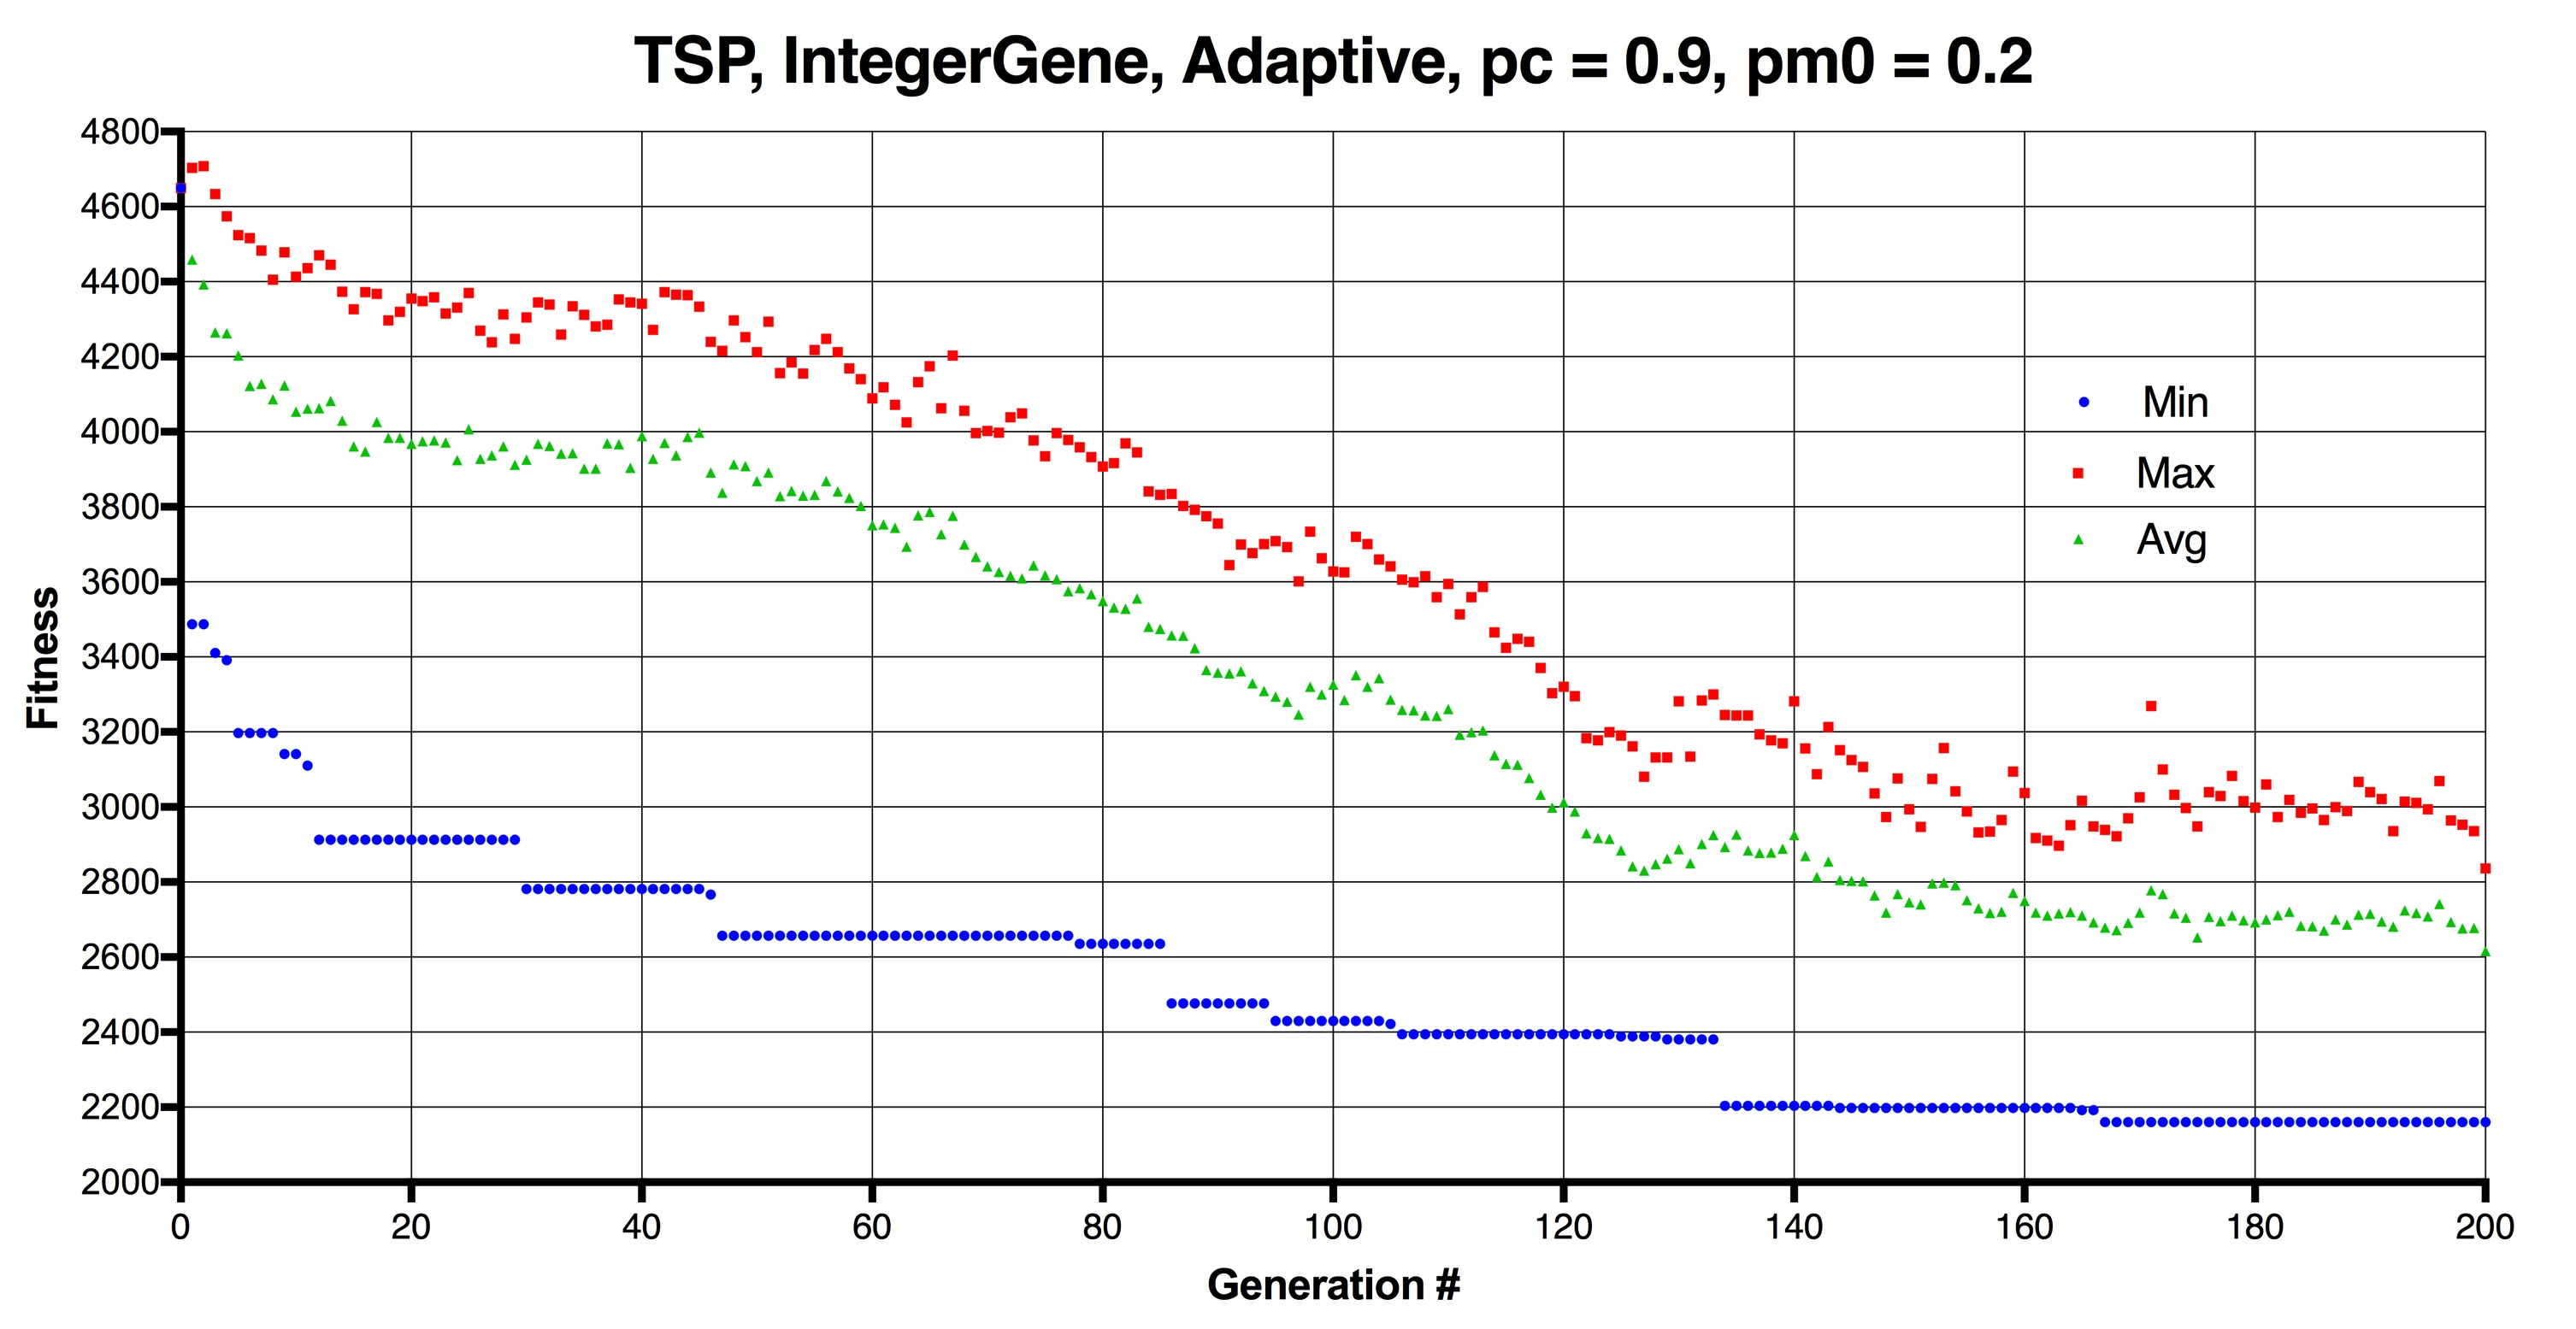
\includegraphics[width=1.0\textwidth]{tsp_02_adaptive.jpg}
    \caption{Evolução do fitness para o problema do Caixeiro Viajante Adaptado Adaptativo, mostrando mínimo, máximo, valor médio e desvio padrão ($p_c=0.9$, ${p_m}_0=0.2$). O menor caminho encontrado tem distância total de 2160.}
    \label{fig:tsp_02_adaptative}
\end{figure}

A curva de interesse aqui foi certamente a da figura \ref{fig:tsp_02_adaptive_pm}. O valor de ${p_m}_0$ não mudou em momento algum, e $p_m$ se estabilizou entorno de seu valor final (0.084). Esta é a curva que melhor demonstra o potencial do AGA desenvolvido aqui: mesmo começando num valor desfavorável para convergência, $p_m$ mudou de patamar e foi estabilizado, trazendo a melhor resposta e a melhor evolução para este problema em 200 gerações.

\begin{figure}[ht!]
    \centering 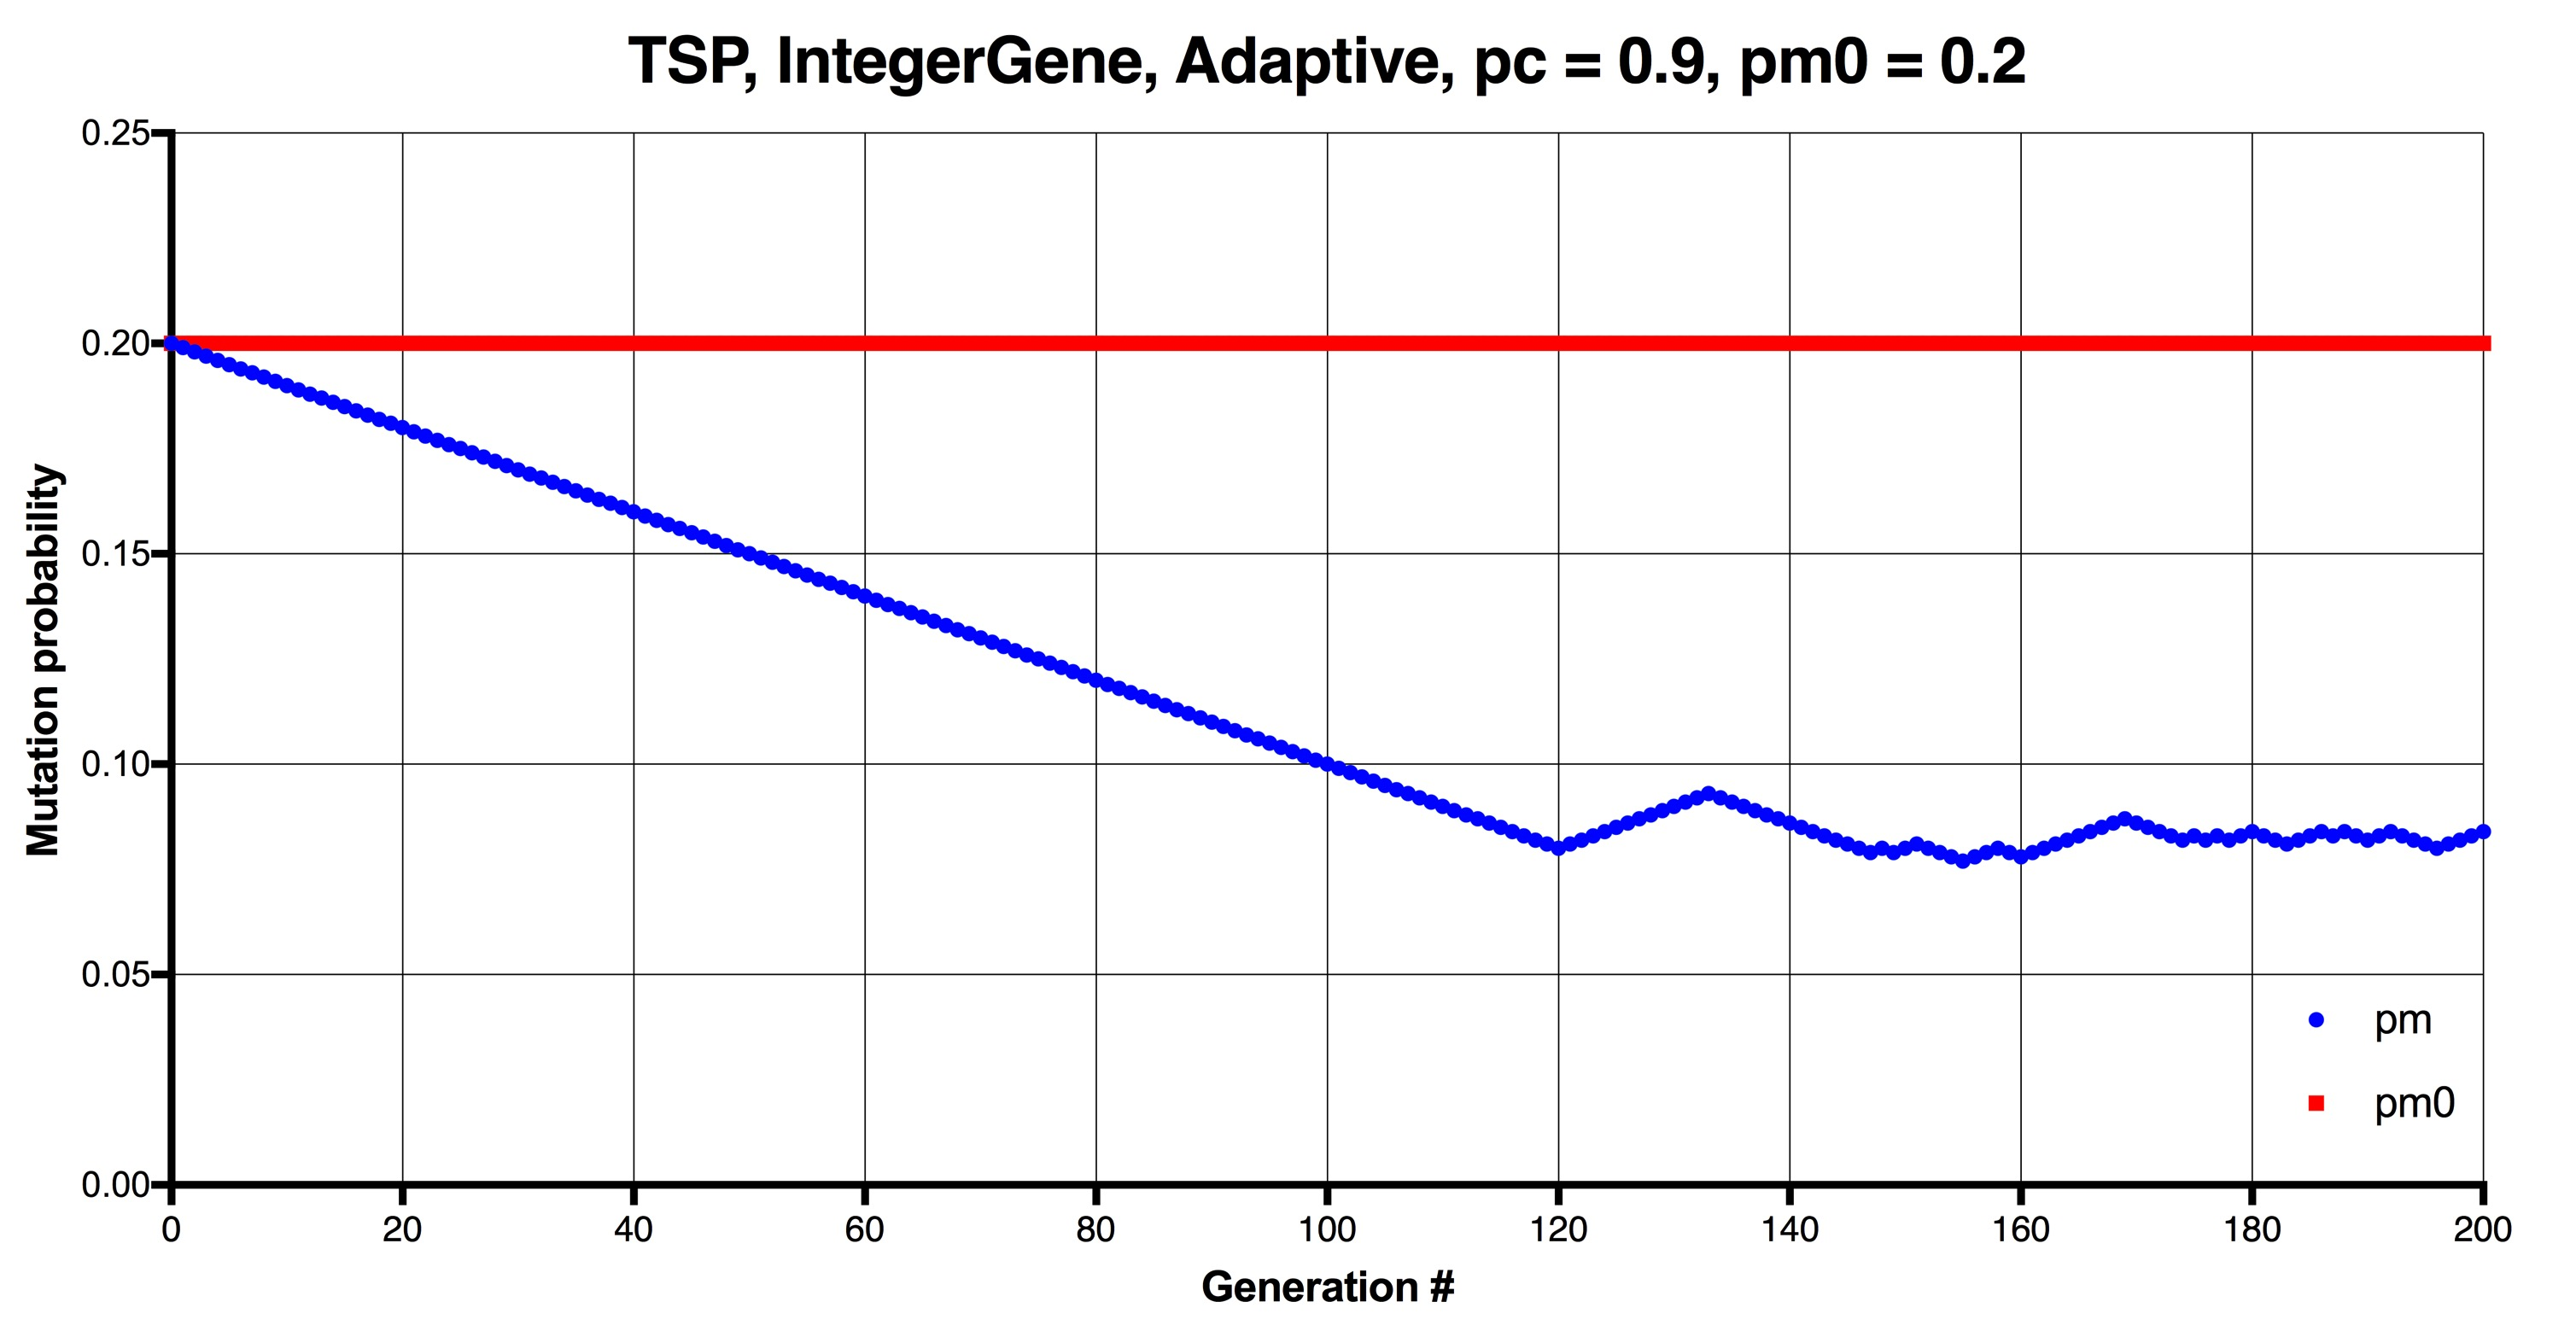
\includegraphics[width=1.0\textwidth]{tsp_02_adaptive_pm.jpg}
    \caption{Probabilidade de mutação ao longo das gerações para o problema do Caixeiro Viajante Adaptado Adaptativo ($p_c=0.9$, ${p_m}_0=0.2$).}
    \label{fig:tsp_02_adaptive_pm}
\end{figure}

Os dados de interesse destas quatro simulações estão presentes na tabela \ref{tab:tsp}.

\begin{table}
\caption{Dados coletados do problema do Caixeiro Viajante Adaptado.}
\label{tab:tsp}

\centering
\begin{tabular}[!hbt]{|c|cc|cc|}
	\hline
	Valor inicial de $p_m$						& \multicolumn{2}{c|}{0.01}		& \multicolumn{2}{c|}{0.2}		\\
	\hline
	Algoritmo analisado (AG = caso estático)	& AG			& AGA			& AG			& AGA			\\
	\hline
	Fitness mínimo após 100 gerações			& $2631$		& $2631$		& $2418$		& $2379$		\\
	Fitness médio após 100 gerações				& $2631$		& $2701.2$		& $3819.5$		& $3267.64$		\\
	Fitness mínimo após 200 gerações 			& $2375$		& $2287$		& $2300$		& $2138$		\\
	Fitness médio após 200 gerações 			& $2375$		& $2349.11$		& $3948.11$		& $2621.33$		\\
	\# máximo de gerações "travado" (mínimo)	& $118 (2631)$	& $69 (2631)$	& $127 (2418)$	& $33 (2661)$	\\
	Valor final de $p_m$						& $0.01$		& $0.043$		& $0.2$			& $0.078$		\\
	Valor mínimo de $p_m$						& $0.01$		& $0.001$		& $0.2$			& $0.072$		\\
	Valor máximo de $p_m$						& $0.01$		& $0.055$		& $0.2$			& $0.204$		\\
	Valor médio de $p_m$						& $0.01$		& $0.0261$		& $0.2$			& $0.122$		\\
	Valor médio de $p_m$ (últimas 100 gerações)	& $0.01$		& $0.0327$		& $0.2$			& $0.0866$		\\
	\hline
\end{tabular}
\end{table}

\section{Discussões}

Os três problemas foram simulados tanto pelo AG estático quanto pelo AGA. Para os problemas OneMax, foi possível observar uma evolução muito melhor para o caso estático do que para o caso adaptativo. Para o problema do Caixeiro Viajante Adaptado, no entanto, observou-se o oposto. Seria possível validar o AGA a partir destes experimentos?

Pensemos nas operações de variação de um AG. Se associarmos probabilidade de crossover $p_c$ (alta) ao fator de homogeneização do fitness da população, então a probabilidade de mutação $p_m$, combinada com elitismo, pode atuar de duas formas:

\begin{itemize}
	\item Tornando a população heterogênea;
	\item \textbf{Melhorando o fitness do melhor indivíduo}.
\end{itemize}

O efeito que será mais predominante dependerá do valor de $p_m$ e do problema. Como visto no OneMax, um valor de 0.01 ou de 0.001 foi suficiente para priorizar o segundo efeito sobre o primeiro, evoluindo gradualmente o melhor indivíduo.

No entanto, o problema do Caixeiro Viajante Adaptado não conseguiu se beneficiar destes efeitos nem para $p_m=0.01$, nem para $p_m=0.2$. Não que o AG estático não possua um valor ideal para convergência deste problema em específico - isto apenas atesta que o parâmetro ideal para um problema pode não ser ideal para outro problema.

Se tentássemos estressar o problema do Caixeiro, poderíamos eventualmente encontrar um valor ideal para ${p_m}_0$. No entanto, tal problema (mesmo adaptado) ainda é NP-Hard, e um valor estático de $p_m$ pode não ser suficiente para encontrar o mínimo global. O que resolveria este problema, quando um valor muito baixo e um valor muito alto de ${p_m}_0$ não são suficientes?

Tal questionamento trouxe a este trabalho a ideia de se usar um algoritmo adaptativo. Algo a se acrescentar ao AG que permitisse adaptar o valor de $p_m$ ao longo das gerações. Mesmo que o uso do AGA não trouxesse melhores soluções mais rapidamente, ele se mostrou melhor para o encontro de percursos cada vez menores. No entanto, o uso do AGA não trouxe o mesmo benefício para os problemas OneMax. Repensar o AGA é uma ideia válida, mas usar o AGA será sempre uma ideia melhor?

Para isso, é necessário considerar os teoremas "No Free Lunch" (NFL - em português, teriam a mesma origem da expressão "Não existe almoço grátis") \cite{wolpert1997no}. De maneira simples, estes teoremas dizem que, para um algoritmo de busca e otimização (como é o caso do AG e do AGA), uma performance elevada para um grupo de problemas (como os problemas OneMax) tem como preço uma queda de performance para todos os outros grupos de problemas (como o problema do Caixeiro Viajante). O AGA tentaria ser a adaptação do AG para se adequar a outros problemas, e mesmo assim, ele veio com uma perda de performance para os problemas OneMax.

Não é possível utilizar o mesmo algoritmo para todos os problemas. Mesmo que não utilizássemos um AGA, ainda haveria formas melhores de se otimizar o AG para um grupo de problemas, incluindo o Caixeiro Viajante. Isso, no entanto, não tira o mérito do AGA.

Pelos experimentos feitos neste trabalho, ele foi capaz de encontrar soluções melhores para um problema mais complexo que os OneMax. Melhor performance é sempre interessante, mas ser capaz de encontrar soluções cada vez melhores sem ficar travado em extremos locais é, ao olhos deste trabalho, um benefício muito melhor. Restaria então verificar se outros problemas conseguiriam se beneficiar do AGA da mesma forma, e se o algoritmo do AGA poderia ser melhorado também.
